\documentclass[11pt, a4paper]{article}
% Shared preamble — SPETC documentation (LuaLaTeX)
\usepackage{fontspec}
\setmainfont{TeX Gyre Termes}
\setsansfont{TeX Gyre Heros}
\setmonofont{TeX Gyre Cursor}
\usepackage{polyglossia}
\setmainlanguage{english}
\usepackage{amsmath, amssymb, mathtools}
\usepackage[final]{microtype}
\usepackage[a4paper, margin=25mm]{geometry}
\usepackage{graphicx}
\usepackage{booktabs}
\usepackage{siunitx}
\sisetup{separate-uncertainty=true}
\usepackage{natbib}
\bibliographystyle{plainnat}
\usepackage[colorlinks=true, linkcolor=blue, citecolor=blue,
            urlcolor=blue, filecolor=blue]{hyperref}
\usepackage{caption}
\captionsetup{font=small, labelfont=bf}
\newcommand{\spetc}{\textsc{spetc}}
\newcommand{\flam}{F_\lambda}
\newcommand{\angstrom}{\text{\AA}}
\newcommand{\code}[1]{\texttt{#1}}


\title{\spetc{} v10: Physics of the Spectro-Photometric\\Exposure Time Calculator}
\author{Mauro Barbieri\\\small\texttt{mauro.barbieri@pm.me}}
\date{2007--2026}

\begin{document}
\maketitle

\begin{abstract}
\spetc{} is an exposure time calculator (ETC) for ground-based broad-band
photometry and low- to high-resolution spectroscopy, descended from the
original Fortran \code{interpola\_spad} chain and rewritten in Python on
\code{astropy}. This document derives every physical relation the code
evaluates: the radiometric chain from a CALSPEC-calibrated template spectrum
to detected photo-electrons; synthetic photometry in the SVO convention;
atmospheric extinction, refraction, airmass and differential dispersion; the
position-dependent night-sky model with van Rhijn airglow, zodiacal light,
integrated starlight and Krisciunas--Schaefer moonlight; Gaussian and Moffat
point-spread functions; the complete noise budget including scintillation and
quantization; slit and slitless (Star Analyser) spectroscopy; and the
treatment of extended sources. Every symbol used in the document is defined
in a dedicated notation section. Version 10.2 adds the physics of the full
audit of the code: full-bandpass slitless sky, resolution-invariant bin
integration of templates, sky-subtraction noise, lunar distance and
zodiacal-elongation dependence, airglow slant-path extinction, telluric
bands, guiding blur, and radial-velocity/reddening template transforms.
Expected performance and the known limits of validity are summarized.
\end{abstract}

\tableofcontents

\section{Introduction}
\label{sec:intro}

An exposure time calculator answers two reciprocal questions: what
signal-to-noise ratio (S/N) a given exposure of a given target will reach, and
how long an exposure is needed to reach a requested S/N. \spetc{} answers both
for broad-band aperture photometry and for slit or slitless spectroscopy, for
any telescope--detector combination the user describes, at any site, time and
sky position.

The code descends from the Fortran \code{interpola\_spad} programs (2007) and
retains their template-calibration convention
(Sect.~\ref{sec:template}), while the physics has been rebuilt in Python on
\code{astropy} \citep{astropy2022}: all radiometric quantities carry explicit
units, all coordinate and time transformations use IERS-based ERFA routines,
and every empirical relation is taken from the published literature cited in
the section where it is used.

Version 10 upgrades the physical model in six areas, each described in its own
section below:
\begin{enumerate}
  \item a position-dependent night-sky model with van Rhijn airglow, zodiacal
        light, integrated starlight, and the \citet{krisciunas1991} moonlight
        model with the published scattering function (Sect.~\ref{sec:sky});
  \item atmospheric refraction and the \citet{pickering2002} airmass
        (Sect.~\ref{sec:airmass});
  \item selectable Gaussian or \citet{moffat1969} point-spread functions
        (Sect.~\ref{sec:psf});
  \item a noise budget extended with \citet{young1967} scintillation,
        \citet{filippenko1982} atmospheric dispersion and ADC quantization
        noise (Sects.~\ref{sec:dispersion}, \ref{sec:noise});
  \item transmission-grating (Star Analyser 100/200) slitless spectroscopy
        (Sect.~\ref{sec:slitless});
  \item extended sources: galaxies, nebulae and planets treated as uniform
        surface brightness (Sect.~\ref{sec:extended}).
\end{enumerate}

Throughout, wavelengths are in \AA{}ngstr\"om internally, fluxes are
$\flam$ in \si{erg.s^{-1}.cm^{-2}.\angstrom^{-1}}, and detected signals are in
photo-electrons. The notation is summarized in Table~\ref{tab:symbols}.

\begin{table}
\centering
\caption{Principal symbols.}
\label{tab:symbols}
\begin{tabular}{ll}
\toprule
Symbol & Meaning \\
\midrule
$\flam$        & spectral flux density [\si{erg.s^{-1}.cm^{-2}.\angstrom^{-1}}] \\
$A$            & unobstructed collecting area $\pi(D^2-d^2)/4$ \\
$T_\lambda$    & filter transmission (0--1) \\
$Q_\lambda$    & detector quantum efficiency (0--1) \\
$\eta$         & scalar optics throughput excluding QE \\
$O_\lambda$    & optional calibrated instrument response curve \\
$T_{\rm atm}(\lambda)$ & zenith atmospheric transmission \\
$X$            & airmass \\
$z$            & zenith distance; $h$ apparent altitude \\
$s$            & seeing FWHM [arcsec] \\
$q$            & parallactic angle \\
$S,B,D$        & source, sky, dark electrons in the aperture \\
$\sigma_R$     & read noise per pixel [e$^-$ rms] \\
$g$            & gain [e$^-$/ADU] \\
$N_{\rm pix}$  & pixels in the photometric aperture or extraction \\
$R$            & resolving power $\lambda/\Delta\lambda$ \\
\bottomrule
\end{tabular}
\end{table}

\section{The measurement chain: how the pieces fit together}
\label{sec:chain}

Before the formula-by-formula derivations, this section tells the story
once, end to end, so that each later section can be read as a close-up of
one link in a chain you have already seen whole.

\subsection{From a magnitude to a spectrum}

The user gives the program one brightness number --- ``the target is
magnitude 12.3 in $V$'' --- but a detector does not respond to
magnitudes; it responds to photons per wavelength. The first task is
therefore to turn one number into a full spectral energy distribution.
This is what the \emph{template} is for: an absolutely calibrated
spectrum of a star of similar type supplies the \emph{shape}
$F_\lambda(\lambda)$, and the magnitude supplies the \emph{level}. The
connection between the two is the synthetic-photometry machinery of
Sect.~\ref{sec:radiometry}: the program computes what magnitude the
template \emph{would} have in the user's reference band, and rescales the
whole spectrum by the ratio to the requested magnitude. Because the
rescaling is total, the template's own flux units are immaterial --- only
its shape and its internal calibration matter --- which is why CALSPEC
standards, surface-brightness planet atlases and arbitrary-unit
supernova models can all serve as templates
(Sect.~\ref{sec:radiometry}). The one number that anchors this step is
the catalogue's $m_{v0}$, the magnitude the template file itself
represents; it is the fulcrum on which the whole calibration turns.

\subsection{From a spectrum above the atmosphere to electrons in a pixel}

The calibrated spectrum then runs the gauntlet of the light path, each
element a multiplicative wavelength-dependent factor inside one integral,
Eq.~(\ref{eq:rate}):

\begin{center}
$F_\lambda$ (target, top of atmosphere)
$\;\rightarrow\; T_{\rm atm}(\lambda)^{X}$ (Sect.~\ref{sec:atmosphere})
$\;\rightarrow\; A\,\eta\,O_\lambda$ (telescope and optics)
$\;\rightarrow\; T_\lambda$ (filter)
$\;\rightarrow\; Q_\lambda$ (detector QE)
$\;\rightarrow\;$ electrons s$^{-1}$
\end{center}

The atmosphere enters twice more, in subtler roles than mere absorption:
it \emph{blurs} (the seeing PSF of Sect.~\ref{sec:psf}, which decides how
much light a finite aperture or slit captures and how bright the peak
pixel gets), it \emph{disperses} (differential refraction,
Sect.~\ref{sec:dispersion}, which drains blue light out of a misaligned
slit), and it \emph{twinkles} (scintillation,
Sect.~\ref{sec:scintillation}, a noise proportional to the signal
itself). And the sky above the site is not dark: the sky model of
Sect.~\ref{sec:sky} --- airglow, zodiacal light, starlight, moonlight,
twilight, or simply the user's SQM reading --- adds its own electrons to
every aperture and every resolution element, through the same instrument
chain.

\subsection{From electrons to a decision}

The last link converts electron counts into the quantities an observer
decides with. The CCD equation, Eq.~(\ref{eq:snr}), combines the source
against every accumulated noise: its own shot noise, the sky's, dark
current, read noise per pixel, scintillation, quantization. Solved
forward it yields the S/N of a given exposure; inverted
(Sect.~\ref{sec:stack}) it yields the exposure for a requested S/N, and,
when that exposure would saturate the brightest pixel --- which the
program predicts independently, from the unextracted PSF peak --- the
stack planner divides it into feasible frames. Spectroscopy adds one
more translation: from S/N per resolution element to the
equivalent-width uncertainty $\sigma(\mathrm{EW})$ of
Sect.~\ref{sec:ew}, which states directly which spectral lines a night
can measure. Everything downstream of the electron counts is exact
bookkeeping; everything upstream is physics with stated approximations
--- the map of which is drawn in Sect.~\ref{sec:expectations}.

\subsection{Where each ingredient comes from}

Every factor in the chain is data the user controls, and each has a
documented file format (User Guide, Sect.~6): the template from the
catalogue; the filter transmission and zero point from an SVO profile
(downloaded or synthesised from a measured curve,
Sect.~\ref{sec:filters}); the QE, optics response and gain table from
the camera's datasheet; the atmospheric transmission from a site FITS
table or the built-in broad-band fallback; the sky level from the
physical model or a hand-held SQM meter. The design intent is that
\emph{nothing physical is hidden in the code}: what the program assumes,
a file or a visible control states, and the run log in the Results
window records.

\section{Notation: every symbol, defined once}
\label{sec:notation}

Every quantity used in this document is defined here, grouped by theme,
with its units and the section where it first does physical work.  Two
deliberate collisions of astronomical convention are flagged explicitly:
$\beta$ denotes both the ecliptic latitude (sky model,
Sect.~\ref{sec:sky}) and the Moffat wing index (PSF, Sect.~\ref{sec:psf});
$\alpha$ denotes both the lunar phase angle (Sect.~\ref{sec:sky}) and the
Moffat core radius (Sect.~\ref{sec:psf}).  The context — sky or PSF —
always disambiguates them, and no equation mixes the two meanings.

\subsection*{Radiometry and magnitudes (Sect.~\ref{sec:radiometry})}

\begin{tabular}{llp{8.6cm}}
\toprule
Symbol & Units & Definition \\
\midrule
$\lambda$ & \si{\angstrom} & Wavelength; all internal grids are in \si{\angstrom}. \\
$\flam(\lambda)$ & \si{erg.s^{-1}.cm^{-2}.\angstrom^{-1}} & Spectral flux
  density per unit wavelength (``F-lambda''), the quantity all templates
  are converted to. \\
$F_\nu$ & Jy & Spectral flux density per unit frequency;
  $1\,\mathrm{Jy} = 10^{-23}\,\si{erg.s^{-1}.cm^{-2}.Hz^{-1}}$. \\
$Z_\nu$ & Jy & The $F_\nu$ zero point of a magnitude system: the flux
  density of a zero-magnitude source (AB: 3631 Jy at every wavelength;
  Vega: per-filter values from the SVO profile). \\
$m$ & mag & Magnitude: $m = -2.5\log_{10}(F/F_{\rm zero})$ in the stated
  system and band. \\
$m_{v0}$ & mag & Catalogue field: the visual magnitude represented by a
  stored template file as shipped (0 for BPGS spectra). \\
$T_\lambda$ & — & Filter (passband) transmission, $0 \le T_\lambda \le 1$. \\
$W_\lambda$ & — & Synthetic-photometry weighting: $\lambda$ for a
  photon-counting detector, 1 for an energy integrator (SVO
  \code{DetectorType}). \\
$Q_\lambda$ & — & Detector quantum efficiency: detected electrons per
  incident photon at $\lambda$. \\
$O_\lambda$ & — & Optics/instrument throughput curve (everything between
  aperture and detector except the filter and QE). \\
$\eta$ & — & Scalar (grey) efficiency factor for losses with no stated
  wavelength dependence. \\
$A$ & \si{cm^2} & Unobstructed collecting area,
  $A = \tfrac{\pi}{4}(D^2 - d_{\rm obs}^2)$, with $D$ the aperture and
  $d_{\rm obs}$ the central-obstruction diameter. \\
$h,\,c$ & cgs & Planck constant and speed of light; $hc/\lambda$ is the
  photon energy. \\
$\dot S,\ \dot B,\ \dot d$ & \si{e^-/s} & Detected electron rates: source
  (aperture- or element-integrated), sky, and dark current per pixel. \\
$v$ & km/s & Radial velocity of the target; positive = receding. \\
$E(B\!-\!V)$ & mag & Interstellar reddening (colour excess); $R_V =
  A(V)/E(B\!-\!V) = 3.1$ assumed; $A(\lambda)$ = extinction in
  magnitudes at $\lambda$ (CCM89 law). \\
\bottomrule
\end{tabular}

\subsection*{Geometry, time and the atmosphere
(Sects.~\ref{sec:atmosphere}, \ref{sec:sky})}

\begin{tabular}{llp{8.6cm}}
\toprule
Symbol & Units & Definition \\
\midrule
$h$ (altitude) & deg & Apparent altitude above the horizon (includes
  refraction unless stated ``geometric''). \\
$z$ & deg & Zenith distance, $z = 90^\circ - h$. \\
$X$ & — & Airmass: the optical path through the atmosphere relative to the
  zenith path; computed from the apparent altitude with
  Eq.~(\ref{eq:pickering}). \\
$T_{\rm atm}(\lambda)$ & — & Zenith atmospheric transmission; the
  transmission at airmass $X$ is $T_{\rm atm}^{\,X}$ (Bouguer law). \\
$k_\lambda$ & mag/airmass & Extinction coefficient;
  $T_{\rm atm} = 10^{-0.4 k_\lambda}$. \\
$n(\lambda)$ & — & Refractive index of air at the site conditions. \\
$\Delta R(\lambda)$ & arcsec & Differential atmospheric refraction
  (atmospheric dispersion) relative to a reference wavelength,
  Eq.~(\ref{eq:dr}). \\
$H,\ \varphi,\ \delta$ & deg & Hour angle of the target, geographic
  latitude of the site, declination of the target. \\
$q$ & deg & Parallactic angle: the position angle of the local vertical at
  the target, measured from North through East, Eq.~(\ref{eq:parallactic}). \\
$P,\ T_{\rm site},\ E$ & hPa, \si{\celsius}, m & Site pressure,
  temperature (ISA defaults from the elevation) and elevation. \\
$t_{\rm exp}$ & s & Exposure time of a single frame. \\
$d_{\rm cm}$ & cm & Telescope aperture diameter (in the scintillation
  law). \\
$\sigma_{\rm scint}/I$ & — & Fractional rms intensity modulation by
  scintillation, Eq.~(\ref{eq:scint}). \\
$s$, FWHM & arcsec & Seeing: the full width at half maximum of the
  seeing-limited stellar profile. \\
$\sigma_g$ & arcsec & Guiding (tracking) error, rms per axis; adds a blur
  of FWHM $2.355\,\sigma_g$ in quadrature to the seeing. \\
$r_0$ & m & Fried parameter of Kolmogorov turbulence;
  seeing $\propto \lambda/r_0$. \\
\bottomrule
\end{tabular}

\subsection*{Sky brightness (Sect.~\ref{sec:sky})}

\begin{tabular}{llp{8.6cm}}
\toprule
Symbol & Units & Definition \\
\midrule
$\mu$ & mag/arcsec$^2$ & Surface brightness: the magnitude of the flux
  received from one square arcsecond of sky. \\
S10 & — & Surface-brightness unit: the equivalent of one star of
  $m_V = 10$ per square degree;
  $\mu = 27.78 - 2.5\log_{10} q$ mag/arcsec$^2$ for a brightness of $q$
  S10 units. \\
nL & — & nanoLambert, the luminance unit of the Krisciunas--Schaefer
  moonlight model; converted to S10 by the factor 3.8. \\
$q_{\rm air},\,q_{\rm zod},\,q_\ast$ & S10 & Airglow, zodiacal-light and
  integrated-starlight brightness components. \\
$a$ & — & Solar-cycle activity, interpolated between tabulated solar
  minima: 0.8 at minimum, 2.0 at maximum. \\
$V(z)$ & — & van Rhijn airglow path-length factor,
  Eq.~(\ref{eq:vanrhijn}). \\
$\hat h$ & km & Height of the airglow emitting layer (90 km). \\
$R_\oplus$ & m & Mean Earth radius, $6.371\times10^6$ m. \\
$\beta$ (sky) & deg & Ecliptic latitude of the field. \\
$b$ & deg & Galactic latitude of the field. \\
$\epsilon$ & deg & Solar elongation of the field: its angular distance
  from the Sun. \\
$\alpha$ (Moon) & deg & Lunar phase angle: $0^\circ$ = full Moon,
  $90^\circ$ = quarter; computed as $180^\circ$ minus the Sun--Moon
  elongation. \\
$\rho$ & deg & Angular separation between the Moon and the target. \\
$I^\ast$ & — & Lunar illuminance factor of the K\&S model. \\
$f(\rho)$ & — & K\&S scattering function (Rayleigh + aureole),
  Eq.~(\ref{eq:ks}). \\
$X_{\rm m}$ & — & Airmass of the Moon. \\
$d_{\rm moon}$ & km & Topocentric distance of the Moon; the illuminance
  scales as $(\bar d/d_{\rm moon})^2$ with $\bar d = 384\,400$ km. \\
$\mu_{\rm SQM}$ & mag/arcsec$^2$ & Zenith $V$ sky brightness measured by
  a Sky Quality Meter. \\
\bottomrule
\end{tabular}

\subsection*{PSF and coupling (Sect.~\ref{sec:psf})}

\begin{tabular}{llp{8.6cm}}
\toprule
Symbol & Units & Definition \\
\midrule
$\sigma$ & arcsec & Gaussian width, $\sigma = \mathrm{FWHM}/2.355$. \\
$\alpha$ (Moffat) & arcsec & Moffat core radius,
  $\alpha = \mathrm{FWHM}/(2\sqrt{2^{1/\beta}-1})$. \\
$\beta$ (Moffat) & — & Moffat wing index; small $\beta$ = strong wings;
  Gaussian is the $\beta \to \infty$ limit. \\
$\mathrm{EE}(r)$ & — & Encircled energy: fraction of the total PSF flux
  inside a circular aperture of radius $r$. \\
$T(w,\delta)$ & — & Slit coupling: fraction of the PSF flux through an
  infinite slit of width $w$ decentred by $\delta$,
  Eq.~(\ref{eq:slit}). \\
$F_\nu$ (CDF) & — & Student-$t$ cumulative distribution with $\nu$
  degrees of freedom (only inside Eq.~\ref{eq:slit}; not a flux). \\
$p$ & arcsec/pixel & Plate scale: $p = 206265\, s_{\rm pix}/f_{\rm tel}$
  with $s_{\rm pix}$ the pixel size and $f_{\rm tel}$ the telescope focal
  length in the same length units. \\
\bottomrule
\end{tabular}

\subsection*{Noise budget and solvers (Sect.~\ref{sec:photometry})}

\begin{tabular}{llp{8.6cm}}
\toprule
Symbol & Units & Definition \\
\midrule
$S,\ B,\ D$ & e$^-$ & Accumulated source, sky and dark charge in the
  aperture over $t_{\rm exp}$. \\
$N_{\rm pix}$ & — & Number of detector pixels summed in the aperture or
  extraction window. \\
$\sigma_R$ & e$^-$ & Read noise per pixel per frame, rms. \\
$g$ & e$^-$/ADU & Conversion gain; the ADC quantization noise is
  $g/\sqrt{12}$ per pixel. \\
$N_{\rm bit}$ & — & ADC bit depth; digital saturation at
  $g\,(2^{N_{\rm bit}}-1)$ electrons. \\
$n_{\rm sky}$ & — & Number of pixels used to \emph{measure} the
  background (sky annulus or slit sky windows); finite $n_{\rm sky}$
  multiplies background variances by $(1 + N_{\rm pix}/n_{\rm sky})$. \\
$\dot b$ & \si{e^-/s}/pixel & Optional extra background rate (detector
  glow, stray light). \\
$C$ & s$^{1/2}$ & Scintillation constant of a configuration:
  $\sigma_{\rm scint}/I = C\,(2 t_{\rm exp})^{-1/2}$. \\
$Q$ & \si{e^-/s} & Total Poisson-like rate in the solver,
  $Q = \dot S + \dot B + \dot D$ (plus the scintillation rate). \\
$\Omega$ & arcsec$^2$ & Angular area of an extended source. \\
$N,\ T$ & —, s & Number of stacked frames and total integration time
  $T = N\,t_{\rm sub}$. \\
\bottomrule
\end{tabular}

\subsection*{Spectroscopy (Sect.~\ref{sec:spectroscopy})}

\begin{tabular}{llp{8.6cm}}
\toprule
Symbol & Units & Definition \\
\midrule
$R$ & — & Resolving power, $R = \lambda/\Delta\lambda$. \\
$\Delta\lambda$ & \si{\angstrom} & Resolution element: the wavelength
  width the instrument cannot subdivide; one output row of the ETC. \\
$\mathcal{D}$ & \si{\angstrom}/pixel & Linear dispersion at the
  detector. \\
$\ell$ & pixel & Line-spread-function FWHM in dispersion-direction
  pixels (slitless: seeing $\oplus$ intrinsic $\oplus$ dispersion
  smear). \\
$n_{\rm mm}$ & mm$^{-1}$ & Grating groove density. \\
$m$ (grating) & — & Diffraction order (1 for the Star Analyser). \\
$L$ & mm & Grating-to-sensor distance of a converging-beam grating. \\
$f_{\rm coll},\ f_{\rm cam}$ & mm & Collimator and camera focal lengths
  of a slit spectrograph. \\
$w_{\rm slit}$ & arcsec & Slit width on the sky. \\
$\delta x$ & \si{\angstrom} & Width of one dispersion pixel,
  $\delta x = \Delta\lambda/(\text{pixels per element})$. \\
$W$ & \si{\angstrom} & FWHM of a spectral line in the Cayrel relation,
  Eq.~(\ref{eq:cayrel}). \\
EW & \si{\angstrom} & Equivalent width: the width of a rectangle of
  continuum height with the same integrated absorption/emission as the
  line. \\
\bottomrule
\end{tabular}

\section{Radiometric framework}
\label{sec:radiometry}

\subsection{Magnitude systems and zero points}

A magnitude $m$ in a system with $F_\nu$ zero point $Z_\nu$ (in Jy)
corresponds to the monochromatic flux density
\begin{equation}
  \flam(\lambda) \;=\; Z_\nu \, \frac{c}{\lambda^2}\; 10^{-0.4\,m},
  \label{eq:flam}
\end{equation}
which the code evaluates with \code{astropy} units
(\code{magnitude\_f\_lambda}). The AB system \citep{oke1983} uses
$Z_\nu = \SI{3631}{Jy}$ at every wavelength; Vega systems use the per-filter
zero points delivered inside each SVO filter profile
\citep{rodrigo2020,bessell1998}.

\subsection{Synthetic photometry (SVO convention)}

The synthetic magnitude of a spectrum $\flam$ in a filter with response
$T_\lambda$ is
\begin{equation}
  m \;=\; -2.5\,\log_{10}
  \frac{\displaystyle\int \flam\,T_\lambda\, W_\lambda\, d\lambda}
       {\displaystyle\int \flam^{\,0}\,T_\lambda\, W_\lambda\, d\lambda},
  \qquad
  W_\lambda = \begin{cases}\lambda & \text{photon counter}\\
                            1 & \text{energy integrator,}\end{cases}
  \label{eq:synthmag}
\end{equation}
where $\flam^{\,0}$ is the zero-magnitude spectrum of
Eq.~(\ref{eq:flam}) and the weighting follows the SVO
\code{DetectorType} flag of the profile. Both conventions are implemented and
regression-tested; for a coloured source they differ measurably.

\subsection{Template calibration}
\label{sec:template}

Template spectra are absolutely calibrated CALSPEC/BPGS spectrophotometry
\citep{bohlin2014}; the catalogue field $m_{v0}$ records the visual magnitude
represented by each file. The code first restores the visual-zero
distribution, $\flam \rightarrow \flam\,10^{0.4 m_{v0}}$ (the original
Fortran convention), then scales it to the user's reference measurement:
\begin{equation}
  \flam^{\rm cal} \;=\; \flam\,10^{0.4 m_{v0}}\;
  10^{-0.4\,\left[m_{\rm ref} - (m_{\rm ref}^{\rm syn}-m_{V}^{\rm syn})\right]},
\end{equation}
where the synthetic colour term $(m_{\rm ref}^{\rm syn}-m_{V}^{\rm syn})$ is
computed from the template itself with Eq.~(\ref{eq:synthmag}) whenever the
reference filter differs from the visual response, and is exactly zero in the
original $V$-only case, which then reduces to the Fortran scale factor
$10^{-0.4(V_{\rm target}-m_{v0})}$.

\subsection{Template sources}

Templates are two-column ASCII or CALSPEC/STScI-style FITS binary tables
(\code{WAVELENGTH}/\code{FLUX}, TUNIT-aware), which admits the whole STScI
reference-atlas family: the CALSPEC standards, the solar-system
surface-brightness atlas, the galactic emission-line atlas, the transient
templates and the CLOUDY planetary-nebula grids. On import, the synthetic
Vega $V$ magnitude of each file is computed against the shipped Bessell.V
profile and stored as the catalogue $m_{v0}$; since the ETC rescales every
template to the entered target magnitude, files with arbitrary or
surface-brightness flux units remain fully usable — only the spectral shape
and the self-consistent $m_{v0}$ matter. Templates that do not fully cover
the $V$ response carry an approximate $m_{v0}$ and should be used with $V$
as the reference filter (the exact same-response path).

\subsection{Detected electron rate}

The photo-electron rate through the full system is
\begin{equation}
  \dot S \;=\; A\,\eta \int
  \flam^{\rm cal}\; T_\lambda\, Q_\lambda\, O_\lambda\,
  T_{\rm atm}(\lambda)^{X}\;
  \frac{\lambda}{hc}\; d\lambda ,
  \label{eq:rate}
\end{equation}
with the trapezoidal quadrature carried out on the filter grid
(photometry) or per resolution element (spectroscopy). Wavelength coverage is
a hard requirement: a template, QE curve, filter or atmospheric table that
does not cover the requested interval raises an error instead of silently
zero-filling.

\section{Atmosphere}
\label{sec:atmosphere}

\subsection{Extinction}

Zenith transmission $T_{\rm atm}(\lambda)$ comes either from a
site-specific FITS table (e.g.\ the Paranal product, whose
\code{EXTINCTION} column in mag\,airmass$^{-1}$ is converted once as
$T=10^{-0.4k_\lambda}$) or from the built-in broad-band $U$--$K$ table
(Table~\ref{tab:sky}). The Bouguer law applies it as $T^{X}$, exactly once,
to the source; observed sky brightnesses are never extinguished a second
time.

\subsection{Refraction and airmass}
\label{sec:airmass}

Apparent altitudes include ERFA atmospheric refraction evaluated at the
ISA pressure and temperature of the site elevation,
$P = \SI{1013.25}{hPa}\,e^{-E/\SI{8435}{m}}$ and
$T = \SI{15}{\celsius} - 0.0065\,E$. The airmass is the
\citet{pickering2002} interpolative formula on the \emph{apparent} altitude
$h$ (degrees),
\begin{equation}
  X \;=\; \frac{1}{\sin\!\big(h + 244/(165 + 47\,h^{1.1})\big)},
  \label{eq:pickering}
\end{equation}
which matches $\sec z$ near the zenith and remains physical to the horizon,
where the plane-parallel form diverges (Fig.~\ref{fig:airmass}). The ETC
deliberately reports no airmass below $h=5^\circ$.

\begin{figure}
  \centering
  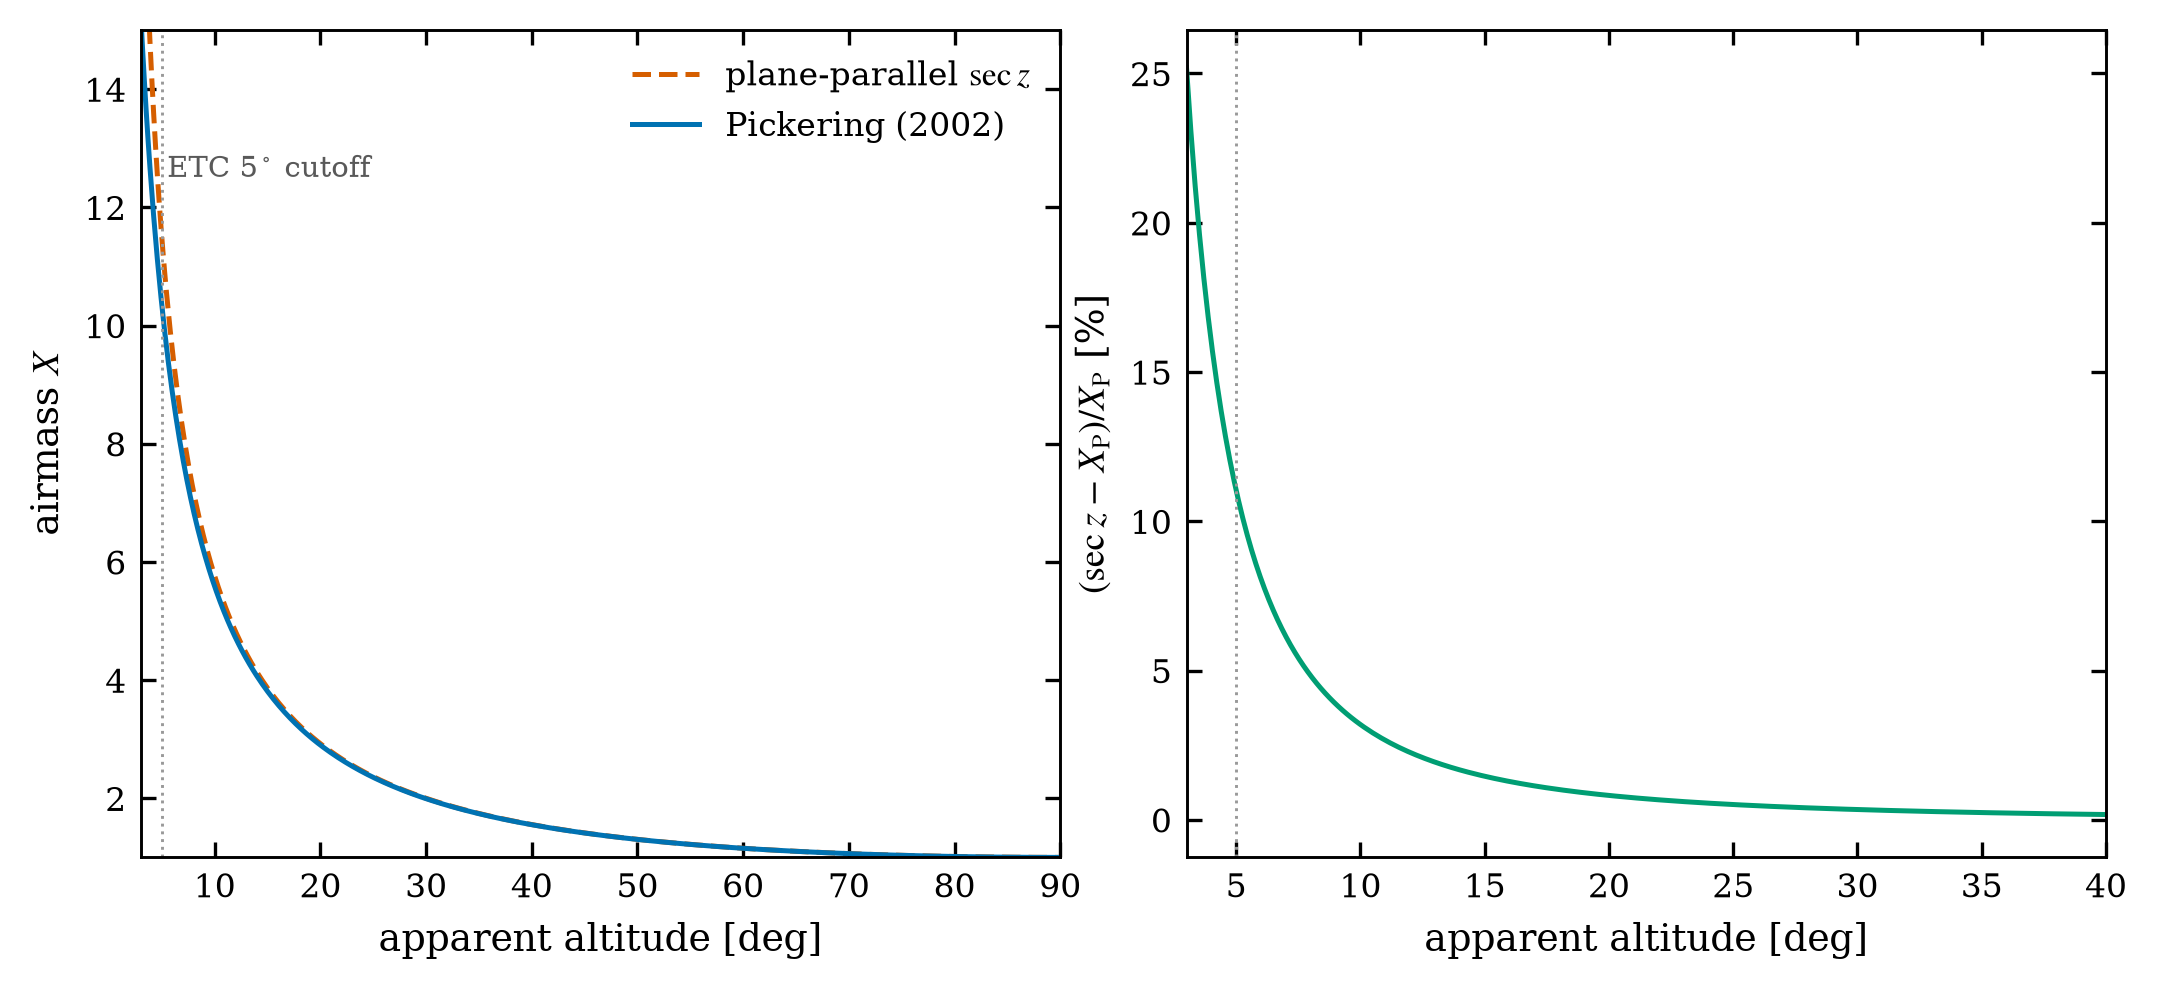
\includegraphics[width=\textwidth]{figures/fig_02_airmass.png}
  \caption{Left: Pickering (2002) airmass versus plane-parallel $\sec z$.
  Right: relative overestimate of $\sec z$; at the ETC's $5^\circ$ cutoff it
  already exceeds 10\%.}
  \label{fig:airmass}
\end{figure}

\subsection{Differential atmospheric refraction}
\label{sec:dispersion}

The refractive index of air follows \citet{filippenko1982}: at standard
conditions
\begin{equation}
  (n-1)\,10^{6} = 64.328 + \frac{29498.1}{146-\sigma^2}
                 + \frac{255.4}{41-\sigma^2},\qquad \sigma = 1/\lambda_{\mu m},
\end{equation}
rescaled to the site pressure and temperature with his equations (2)--(3),
including the water-vapour term. The differential refraction relative to a
reference wavelength is
\begin{equation}
  \Delta R(\lambda) = 206265\,\big[n(\lambda)-n(\lambda_{\rm ref})\big]\tan z ,
  \label{eq:dr}
\end{equation}
about $1''$ between 4000 and \SI{5500}{\angstrom} at $z=45^\circ$
(Fig.~\ref{fig:dispersion}). Its use in slit losses is described in
Sect.~\ref{sec:slit}; the parallactic angle
\begin{equation}
  q \;=\; \arctan\!\frac{\sin H}{\tan\varphi\cos\delta - \sin\delta\cos H}
  \label{eq:parallactic}
\end{equation}
($H$ hour angle, $\varphi$ latitude, $\delta$ declination) is reported for
every time sample, because a slit oriented at $q$ suffers no dispersion
loss.

\begin{figure}
  \centering
  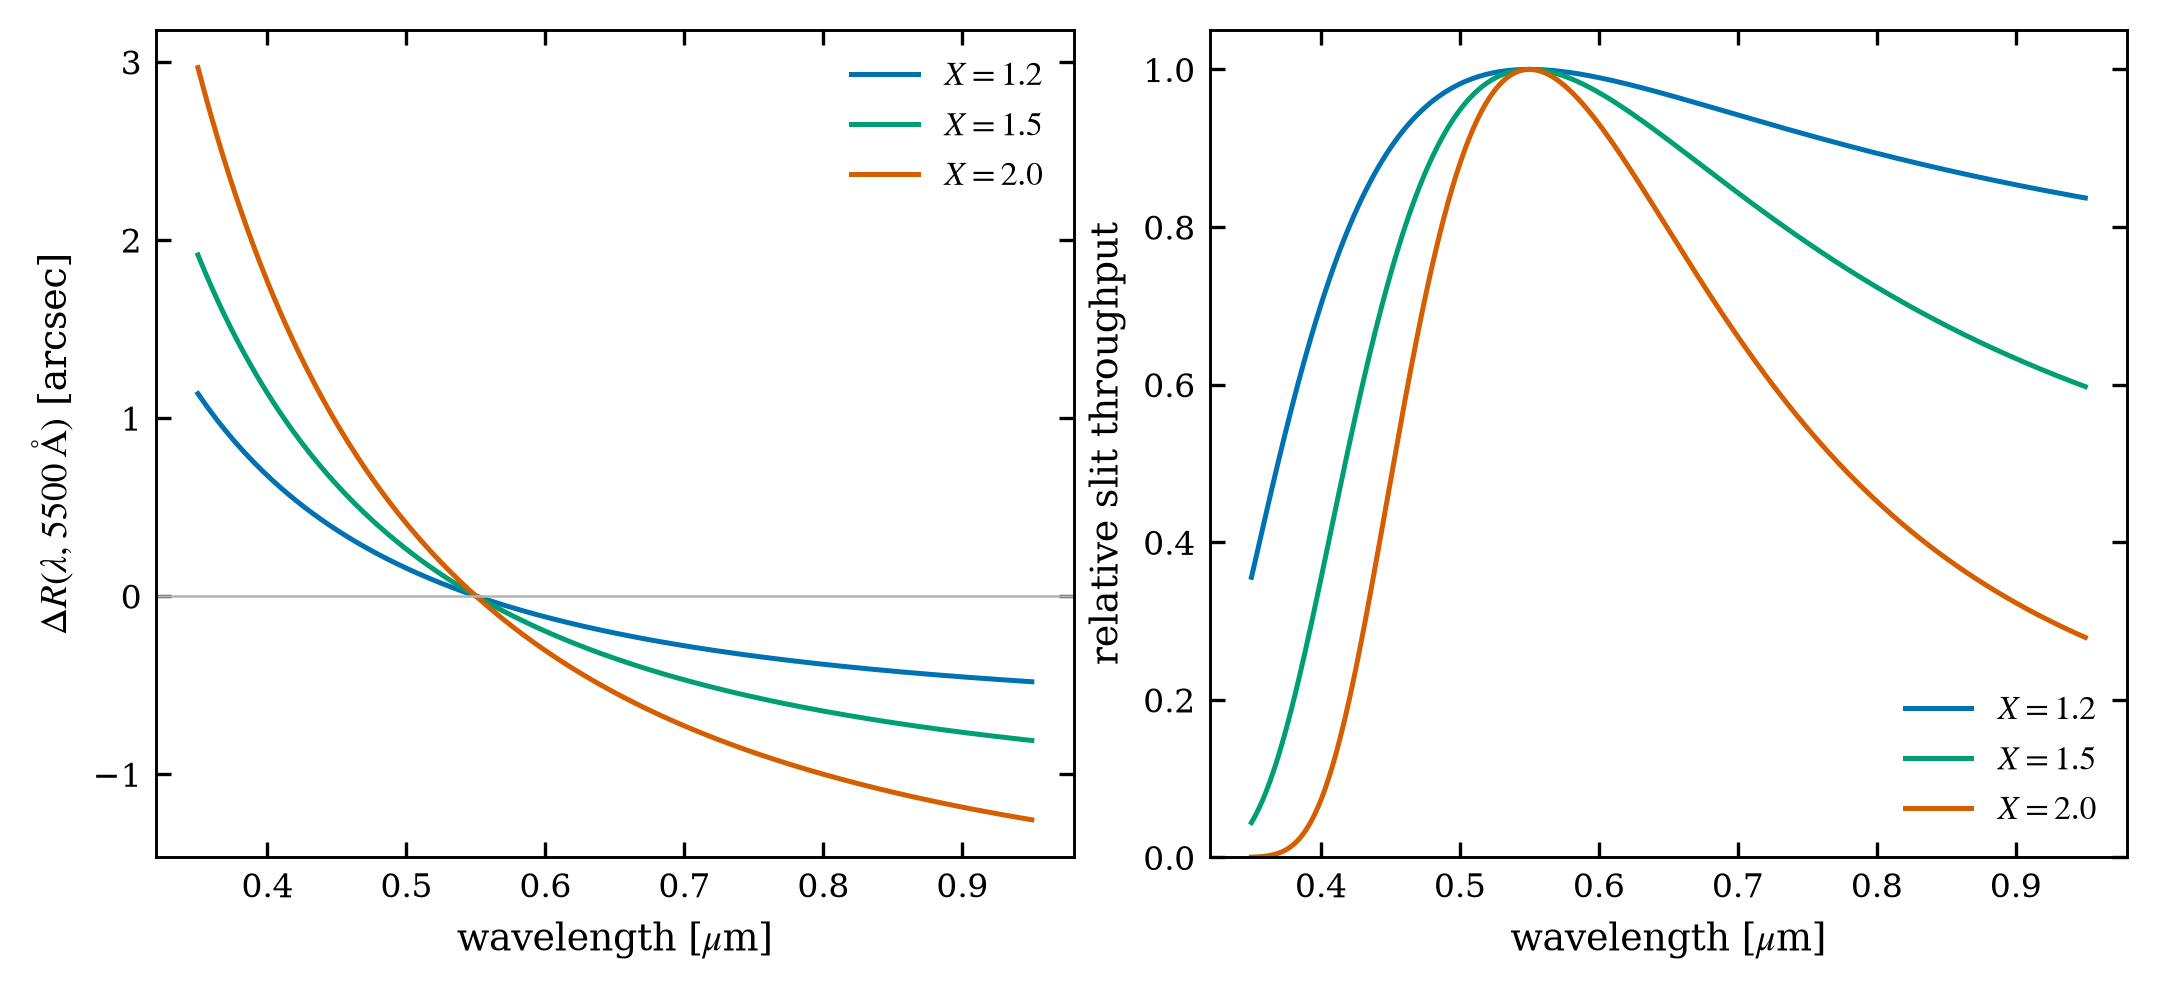
\includegraphics[width=\textwidth]{figures/fig_05_dispersion.png}
  \caption{Left: differential refraction relative to \SI{5500}{\angstrom}
  for three airmasses. Right: resulting relative slit throughput for a
  $1.5''$ slit in $1.5''$ seeing when the slit is \emph{not} at the
  parallactic angle (worst-case geometry).}
  \label{fig:dispersion}
\end{figure}

\subsection{Scintillation}
\label{sec:scintillation}

Intensity scintillation follows the \citet{young1967} law, kept in the
functional form endorsed by \citet{osborn2015},
\begin{equation}
  \frac{\sigma_{\rm scint}}{I} \;=\;
  0.09\; d_{\rm cm}^{-2/3}\, X^{1.75}\,
  e^{-E/\SI{8000}{m}}\,(2\,t_{\rm exp})^{-1/2},
  \label{eq:scint}
\end{equation}
with $d$ the aperture diameter, $E$ the site elevation and $t_{\rm exp}$
the exposure time. Because this noise is multiplicative in the source flux,
it dominates bright-star photometry and imposes a hard S/N ceiling
$\simeq I/\sigma_{\rm scint}$ per exposure (Fig.~\ref{fig:snrbudget}).

\section{Night-, twilight- and day-sky model}
\label{sec:sky}

For faint targets the sky, not the detector, is the adversary: once the
background electrons in the aperture outnumber the source electrons, the
S/N grows only as the square root of exposure time and every magnitude of
extra sky brightness costs a factor 2.5 in required time. An ETC is
therefore only as honest as its sky model. \spetc{}'s model has an
unusual property for a tool in this class: it is \emph{position- and
time-dependent}. The same target yields a different sky --- and a
different exposure recommendation --- depending on where it sits with
respect to the ecliptic (zodiacal light), the Milky Way (integrated
starlight), the Moon (scattered moonlight), the Sun (twilight), and the
local zenith (airglow path length), all evaluated per time sample of the
night. The components and their assembly are as follows.

\subsection{Dark sky}

Surface brightnesses are budgeted in \emph{S10 units} — the brightness
equivalent to one star of visual magnitude 10 per square degree, a linear
(flux-like) unit in which components simply add; the conversion to
magnitudes per square arcsecond is $\mu = 27.78 - 2.5\log_{10}q$ for a
brightness of $q$ S10. The dark-sky normalization is the broad-band
$U$--$K$ surface-brightness table of Table~\ref{tab:sky} (from the ING
model of \citealt{bennellison1998}), corrected for the pointing and epoch
through the S10 component budget
\begin{equation}
  q_3 \;=\; q_{\rm air}\,V(z)\,\mathcal{E}(z) \;+\;
            q_{\rm zod}(|\beta|)\,g(\epsilon) \;+\; q_\ast(|b|),
\end{equation}
normalized to the dark reference composition $q_{\rm ref} = 145 + 60$ S10.
The components are:
\begin{itemize}
\item \textbf{Airglow}: $q_{\rm air} = 145 + 130\,(a-0.8)/1.2$ S10, where the
  solar-cycle activity $a \in [0.8, 2.0]$ is interpolated between the
  tabulated solar minima (airglow is excited by solar UV, so it roughly
  doubles from solar minimum to maximum). The line-of-sight enhancement is
  the van Rhijn path-length law \citep{vanrhijn1921} for an emitting layer
  at height $\hat h = \SI{90}{km}$,
  \begin{equation}
    V(z) = \Big[1 - \Big(\tfrac{R_\oplus}{R_\oplus+\hat h}\sin z\Big)^2\Big]^{-1/2},
    \label{eq:vanrhijn}
  \end{equation}
  which is sub-linear in airmass and bounded ($V \simeq 6$) at the horizon
  (Fig.~\ref{fig:skypos}, right). The raw van Rhijn factor is however
  never observed: the emitted light must still descend through the
  troposphere along the same slant, which attenuates it by
  \begin{equation}
    \mathcal{E}(z) \;=\; 10^{-0.4\,k_V\,[X_{\rm KY}(z) - 1]},
  \end{equation}
  with $k_V$ the $V$ extinction coefficient and $X_{\rm KY}$ the
  \citet{kasten1989} line-of-sight airmass
  $[\cos z + 0.50572\,(96.07995-z)^{-1.6364}]^{-1}$, finite
  ($X \simeq 38$) at the horizon. Near the horizon $\mathcal{E}$
  partially cancels the van Rhijn enhancement, matching the observed
  behaviour (v10.2).
\item \textbf{Zodiacal light} — sunlight scattered by interplanetary
  dust: $q_{\rm zod} = 140 - 90 \sin|\beta|$ S10 for
  $|\beta| < 60^\circ$, else 60 S10, symmetric about the ecliptic. This
  latitude law describes the anti-solar sky; towards the Sun the dust
  column and the scattering efficiency both rise steeply. The solar
  elongation $\epsilon$ (the field's angular distance from the Sun)
  therefore multiplies it by the factor
  \begin{equation}
    g(\epsilon) \;=\;
    \begin{cases}
      (\epsilon/110^\circ)^{-2.3} & 30^\circ \le \epsilon < 110^\circ\\
      1 & \epsilon \ge 110^\circ,
    \end{cases}
  \end{equation}
  a power-law fit to the \citet{leinert1998} tables at $\beta = 0$
  ($\sim$4$\times$ brighter at $\epsilon = 60^\circ$); below $30^\circ$
  the line of sight is unobservable and the factor is held (v10.2).
\item \textbf{Integrated starlight} — the summed light of unresolved
  stars: $q_\ast = 100\,e^{-|b|/10^\circ}$ S10, falling away from the
  galactic plane.
\end{itemize}
The field's ecliptic and galactic latitudes are computed from the entered
ICRS coordinates with \code{astropy}; the sky is therefore genuinely
position-dependent (Fig.~\ref{fig:skypos}, left).

\begin{table}
\centering
\caption{Built-in broad-band sky data ($U$--$K$): dark-sky surface
brightness, extinction coefficient, Vega zero point and
Krisciunas--Schaefer lunar colour factor.}
\label{tab:sky}
\begin{tabular}{lccccc}
\toprule
Band & $\lambda$ [\si{\angstrom}] & $\mu_{\rm dark}$ [mag/$''^2$] &
$k$ [mag/X] & $Z_\nu^{\rm Vega}$ [Jy] & lunar factor \\
\midrule
$U$ &  3650 & 22.0 & 0.550 & 1810 &  2.00 \\
$B$ &  4450 & 22.7 & 0.250 & 4260 &  1.60 \\
$V$ &  5510 & 21.9 & 0.150 & 3640 &  2.40 \\
$R$ &  6580 & 21.0 & 0.090 & 3080 &  3.00 \\
$I$ &  8060 & 20.0 & 0.060 & 2550 &  5.90 \\
$Z$ & 10000 & 18.8 & 0.050 & 2250 &  8.94 \\
$J$ & 12500 & 16.1 & 0.100 & 1594 & 13.06 \\
$H$ & 16500 & 14.7 & 0.110 & 1024 & 18.09 \\
$K$ & 22000 & 12.5 & 0.070 &  667 & 24.04 \\
\bottomrule
\end{tabular}
\end{table}

\begin{figure}
  \centering
  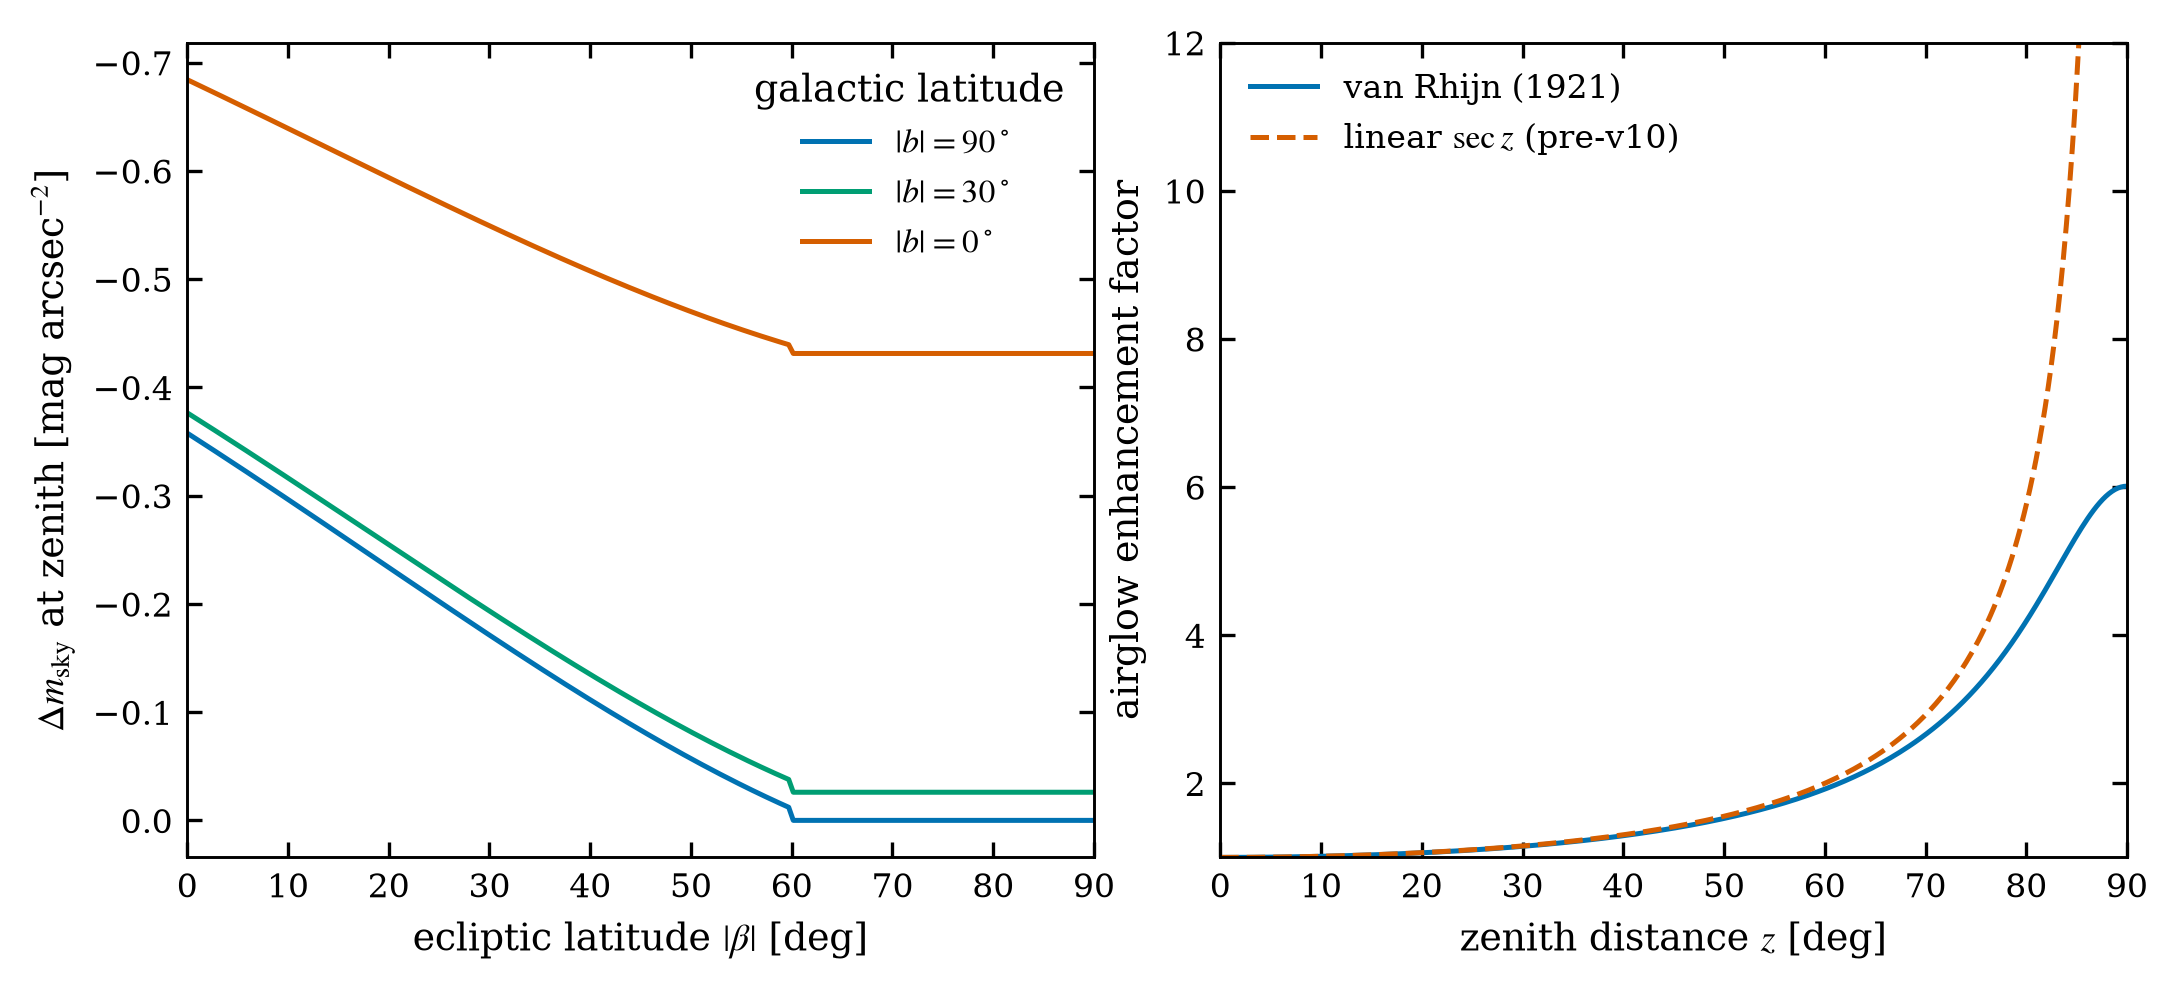
\includegraphics[width=\textwidth]{figures/fig_04_sky_position.png}
  \caption{Left: zenith dark-sky brightening relative to the tabulated
  values as a function of ecliptic latitude, for three galactic latitudes
  (solar minimum). Right: van Rhijn airglow enhancement versus the linear
  $\sec z$ scaling used before v10.}
  \label{fig:skypos}
\end{figure}

\subsection{Moonlight}

Moonlight follows \citet{krisciunas1991}. The lunar phase angle $\alpha$
is the Sun--Moon--Earth angle ($0^\circ$ = full Moon, $90^\circ$ =
quarter), computed as $180^\circ$ minus the Sun--Moon elongation. The
lunar illuminance — the flux of moonlight arriving at the top of the
atmosphere — is
$I^\ast = 10^{-0.4(3.84 + 0.026|\alpha| + 4\times10^{-9}\alpha^4)}
\,(\bar d/d_{\rm moon})^2$: the polynomial is K\&S's fit to the lunar
phase curve, and the second factor is the inverse-square modulation by
the topocentric Moon distance $d_{\rm moon}$ around its mean
$\bar d = 384\,400$ km — a $\pm 15\%$ brightness swing over the
anomalistic month that the track supplies per time sample (v10.2). The
scattering function at Moon--target separation $\rho$ is
\begin{equation}
  f(\rho) \;=\; 10^{5.36}\big(1.06 + \cos^2\rho\big) \;+\;
                 10^{6.15 - \rho/40^\circ}.
  \label{eq:ks}
\end{equation}
The scattering function has two physically distinct terms:
$10^{5.36}(1.06+\cos^2\rho)$ is the Rayleigh contribution (molecular
scattering, with its characteristic $1+\cos^2$ angular pattern), and
$10^{6.15-\rho/40^\circ}$ is the aerosol \emph{aureole}, the forward-scattering
halo around the Moon. The moonlit surface brightness in nanoLambert (a
luminance unit; 1 nL converts to 3.8 S10) is
$B_{\rm moon} = I^\ast f(\rho)\,
10^{-0.4kX_{\rm m}}\big(1 - 10^{-0.4kX}\big)$, where $X_{\rm m}$ is the
Moon's airmass (the moonlight is first extinguished on its way down) and
the bracket is the fraction of light scattered \emph{out of} the direct
beam along the target's path — the scattered moonlight the target line of
sight picks up. This is converted to S10 and
distributed over the nine bands with the lunar colour factors of
Table~\ref{tab:sky}. Equation~(\ref{eq:ks}) corrects a long-standing
transcription error in which the constant $10^{5.36}$ appeared inside the
exponent; the two forms diverge by more than three orders of magnitude
within $30^\circ$ of the Moon (Fig.~\ref{fig:ks}).

\begin{figure}
  \centering
  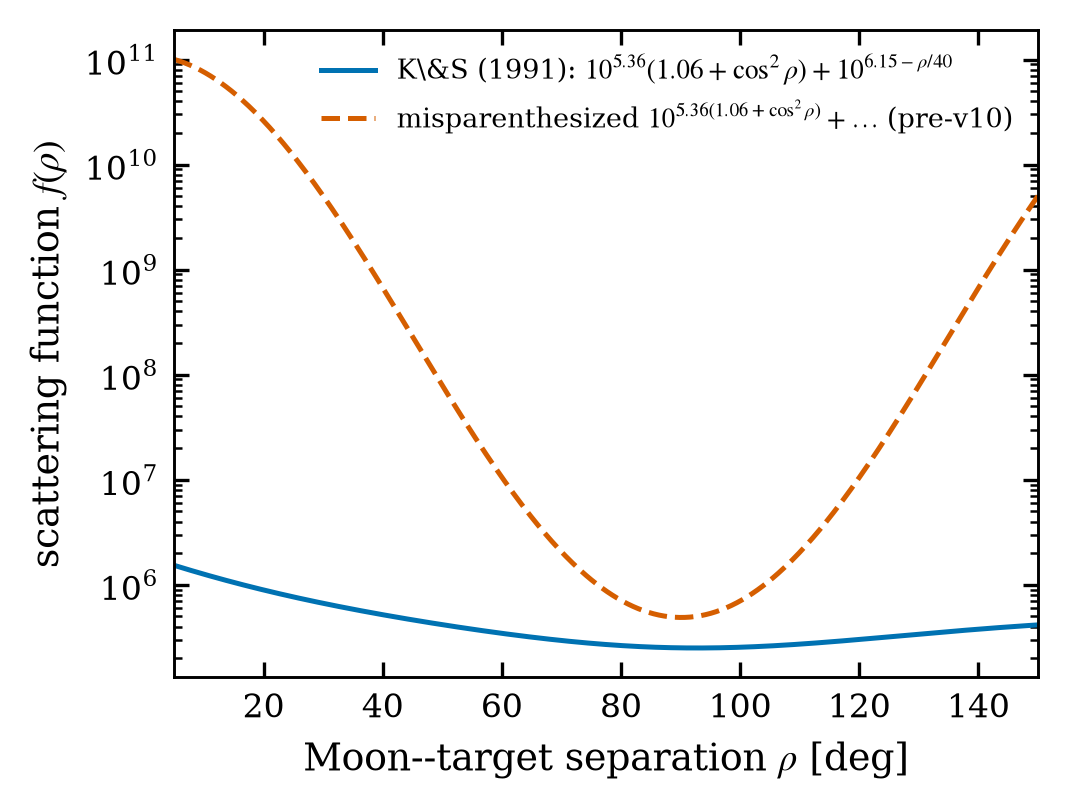
\includegraphics[width=0.62\textwidth]{figures/fig_01_moon_scattering.png}
  \caption{The \citet{krisciunas1991} scattering function (solid) and the
  misparenthesized variant present before v10 (dashed).}
  \label{fig:ks}
\end{figure}

\subsection{SQM and Bortle input}
\label{sec:sqm}

Amateur observers know their sky as a Sky Quality Meter reading (zenith
$V$ surface brightness) or a \citet{bortle2001} class rather than as a
per-band table. In \code{sqm} mode the entered zenith SQM value $\mu_{\rm
SQM}$ replaces the dark-sky normalization directly:
\begin{equation}
  \mu(\lambda_{\rm piv}) \;=\; \mu_{\rm SQM} \;+\;
  \big[\mu_{\rm tab}(\lambda_{\rm piv}) - \mu_{\rm tab}(V)\big],
\end{equation}
i.e.\ the built-in table supplies only the band colour, while the SQM
reading — which already contains the site's light pollution and current
airglow — sets the level. The Krisciunas--Schaefer Moon contribution of
the previous subsection is applied on top unchanged. A Bortle-class
selector fills typical zenith SQM values (21.9, 21.8, 21.6, 21.1, 20.5,
19.8, 19.0, 18.0, 17.0 mag\,arcsec$^{-2}$ for classes 1--9).

\subsection{Twilight and daylight}
\label{sec:daylight}

Between \emph{geometric} Sun altitudes of $-18^\circ$ (end of
astronomical twilight) and $0^\circ$ the dark and daylight skies are
blended linearly in flux — magnitudes cannot be averaged, fluxes can.
Above the horizon a daylight table in the \citet{weaver1947} lineage
supplies the $V$-band surface brightness as a function of solar and sky
zenith distance, mapped to other bands with the dark-sky colours of
Table~\ref{tab:sky}.

The v10.1 physics audit found the daylight table, read directly as
mag/arcsec$^2$, to be $\sim$4.5 magnitudes too \emph{faint}: its values
(8.5--9.2) would make the daytime sky only $\sim$200$\times$ brighter
than a dark night, whereas the physical clear daytime zenith sky is
$\sim$3000--8000 cd/m$^2$, i.e.\ $V \simeq 3.5$--4.5 mag/arcsec$^2$
against the night-sky anchor (21.9 mag/arcsec$^2 \approx
2\times10^{-4}$ cd/m$^2$) — a $\sim$$10^7$ flux ratio. The v10.2 model
therefore keeps the table's \emph{shape} in solar and sky zenith
distance but re-anchors its brightest entry to the physical
$V = 4.0$ mag/arcsec$^2$; the twilight blend inherits the corrected
anchor. Both regimes remain broad-band approximations, clearly flagged
in the user interface, and the original supplied table is preserved in
the source for the day the exact Weaver unit conversion is re-derived.

\section{Point-spread function and aperture coupling}
\label{sec:psf}

The point-spread function is the currency in which three different
questions are paid: how much of a star's light enters a photometric
aperture of a given radius, how much passes a slit of a given width and
decentring, and how much lands on the single brightest pixel (the
saturation question). All three are integrals of the same profile over
different domains, and all three are sensitive to the profile's
\emph{wings}: real seeing profiles carry far more energy at large radii
than a Gaussian of the same FWHM, which makes Gaussian-based aperture
corrections optimistic and Gaussian-based saturation predictions
slightly pessimistic. \spetc{} therefore offers both the Gaussian (for
comparability with other tools) and the Moffat profile (for realism),
everywhere through analytic expressions --- no PSF is ever rendered or
numerically integrated, which keeps the whole-night time series fast.

The seeing-limited PSF is selectable between a circular Gaussian and a
circular \citet{moffat1969} profile
\begin{equation}
  I(r) \propto \Big(1 + \frac{r^2}{\alpha^2}\Big)^{-\beta},
  \qquad
  \alpha = \frac{\rm FWHM}{2\sqrt{2^{1/\beta}-1}},
\end{equation}
whose power-law wings ($\beta \simeq 2.5$--$4.7$; the Gaussian is the
$\beta\to\infty$ limit) reproduce real seeing profiles that a Gaussian
underestimates.

\paragraph{Encircled energy.} For a circular aperture of radius $r$,
\begin{equation}
  \mathrm{EE}_{\rm Gauss}(r) = 1 - e^{-r^2/2\sigma^2},
  \qquad
  \mathrm{EE}_{\rm Moffat}(r) = 1 - \Big(1+\frac{r^2}{\alpha^2}\Big)^{1-\beta}.
\end{equation}

\paragraph{Slit coupling.} The flux through an infinite slit of width $w$
whose centre is displaced by $\delta$ from the PSF centroid uses the
one-dimensional marginal profile. For the Gaussian this is the usual error
function; for the circular Moffat the marginal is \emph{exactly} a Student-$t$
distribution with $\nu = 2\beta-2$ degrees of freedom and scale
$\alpha/\sqrt{\nu}$, so
\begin{equation}
  T(w,\delta) \;=\;
  F_\nu\!\Big(\frac{w/2-\delta}{\alpha/\sqrt{\nu}}\Big) -
  F_\nu\!\Big(\frac{-w/2-\delta}{\alpha/\sqrt{\nu}}\Big),
  \label{eq:slit}
\end{equation}
with $F_\nu$ the Student-$t$ CDF --- no numerical integration is required.
The same expression with $w$ equal to one pixel gives the central-pixel
fraction used for saturation prediction, as the separable product of the
dispersion and spatial couplings. Figure~\ref{fig:psf} compares the models.

\begin{figure}
  \centering
  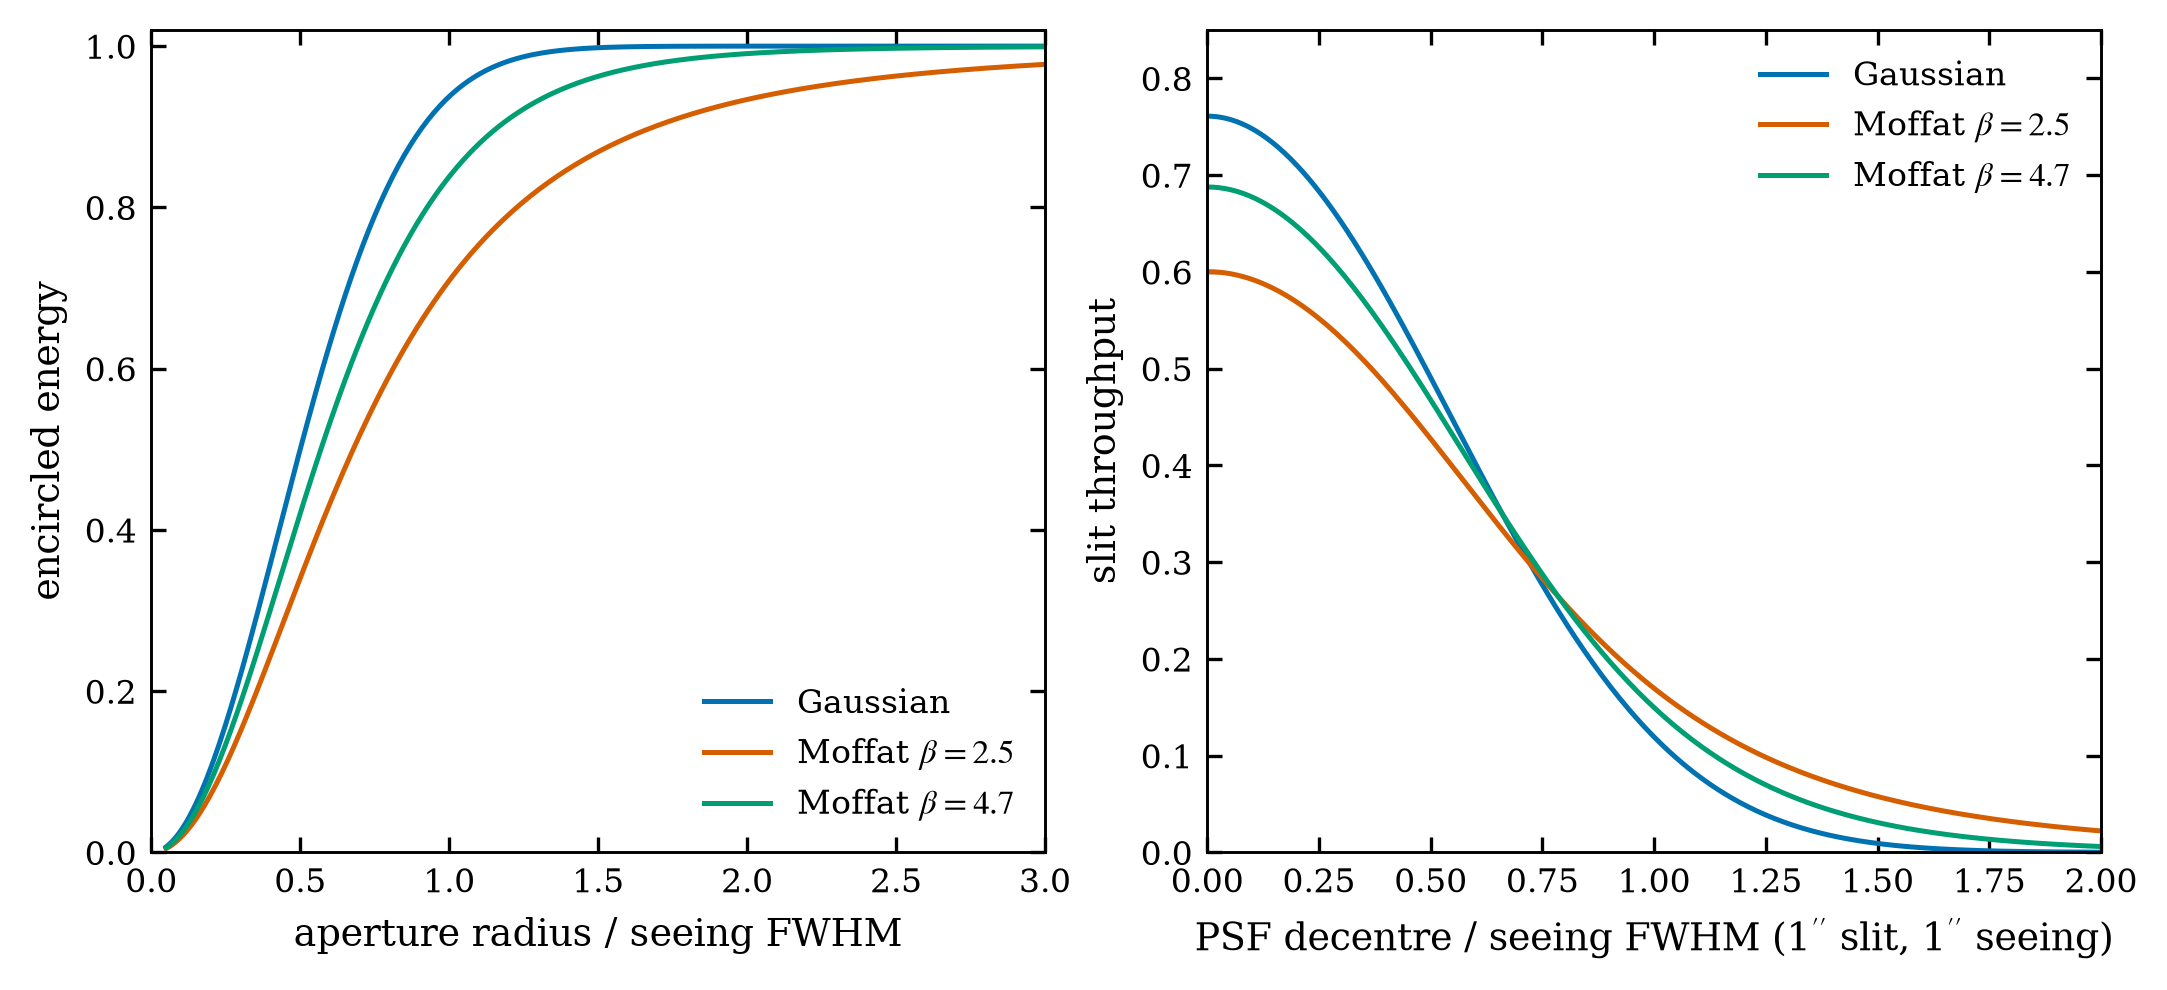
\includegraphics[width=\textwidth]{figures/fig_03_psf.png}
  \caption{Left: encircled energy versus aperture radius in units of the
  seeing FWHM. Right: slit throughput of a slit of one seeing-FWHM width as
  the PSF is decentred, Eq.~(\ref{eq:slit}); the Moffat wings both lower the
  centred coupling and soften the decentring penalty.}
  \label{fig:psf}
\end{figure}

\subsection{Wavelength and airmass dependence of the seeing}
\label{sec:seeing-scaling}

The seeing FWHM is not a constant of the night: Kolmogorov turbulence gives
a Fried parameter $r_0 \propto \lambda^{6/5}(\cos z)^{3/5}$ and hence a
seeing FWHM $\propto \lambda/r_0$,
\begin{equation}
  \mathrm{FWHM}(\lambda, X) \;=\; s_{V,\rm zenith}\;
  X^{0.6}\;\Big(\frac{\lambda}{5000\,\text{\AA}}\Big)^{-0.2},
  \label{eq:seeing-scaling}
\end{equation}
where $s_{V,\rm zenith}$ is the entered zenith seeing in $V$ and $X$ the
airmass. This is the exact form used by ETC-42
\citep[CeSAM/LAM,][\code{calculator/psf/Seeing.java}]{etc42}. As an
optional mode, \spetc{} applies Eq.~(\ref{eq:seeing-scaling}) per wavelength
in the spectroscopic slit and extraction couplings (so blue light suffers
larger losses than red through the same slit), and at the observing band's
pivot wavelength in photometry. Because the airmass factor is evaluated per
time sample, the whole-night time series then correctly shows the seeing ---
and the losses that follow from it --- degrading as the target sets. The
mode is off by default, leaving the seeing flat; when it is on, the entered
value is by definition the zenith $V$ seeing.

\subsection{Guiding blur}
\label{sec:guiding}

Over a long exposure the star also moves: periodic error, polar-alignment
drift and guiding corrections smear the image. If the tracking error is
approximately Gaussian with rms $\sigma_g$ per axis, the time-averaged
image is the seeing profile convolved with a Gaussian of FWHM
$2.355\,\sigma_g$, and the effective image width entering every coupling
of this section is
\begin{equation}
  \mathrm{FWHM}_{\rm eff} \;=\;
  \sqrt{\mathrm{FWHM}_{\rm seeing}^2 + (2.355\,\sigma_g)^2}.
\end{equation}
An entered guiding rms of 0 (the default) reproduces the pure-seeing
case; a typical unguided minute on a mid-range mount
($\sigma_g \sim 1''$) visibly lowers aperture and slit couplings, which
is exactly the effect amateurs observe between guided and unguided
frames (v10.2).

\subsection{Defocused PSF: the geometric donut}
\label{sec:defocus}

Defocused photometry spreads a bright star deliberately over many pixels to
suppress scintillation, flat-field residuals and saturation. When the
detector is displaced by a distance $\delta$ from the focal plane, the
geometric image of a point source is the projection of the (annular) pupil:
a uniformly-illuminated ring, or ``donut''. For a primary of diameter $D$
and focal length $F$ (focal ratio $N = F/D$), similar triangles give a blur
circle of full diameter $\delta/N = \delta D/F$, i.e.\ an outer radius on the
focal plane
\begin{equation}
  r_{\rm out} \;=\; \frac{\delta D}{2F},
\end{equation}
which depends only on $|\delta|$: intra- and extra-focal displacements of
equal magnitude give identical images. A central obstruction of linear
fraction $\varepsilon = D_{\rm obs}/D$ (a classical Ritchey--Chr\'etien or
Cassegrain, $\varepsilon>0$) blocks the inner cone and leaves a hole of
radius $r_{\rm in} = \varepsilon\,r_{\rm out}$; a classical reflector modelled
with $\varepsilon = 0$ gives a filled disc. A uniformly illuminated pupil maps,
in the geometric limit, to a flat annulus, so the encircled energy is analytic:
\begin{equation}
  \mathrm{EE}(r) \;=\;
  \begin{cases}
    0, & r < r_{\rm in},\\[2pt]
    \dfrac{r^2 - r_{\rm in}^2}{r_{\rm out}^2 - r_{\rm in}^2}, & r_{\rm in} \le r \le r_{\rm out},\\[8pt]
    1, & r > r_{\rm out}.
  \end{cases}
\end{equation}
Focal-plane radii convert to angle through the plate scale
($\SI{1}{\micro\metre} \to 206264.8\times10^{-3}/F_{\rm mm}$ arcsec) and to
pixels through the pixel pitch. The user selects a photometry aperture radius
$r_{\rm ap}$ from this curve; the captured light fraction is
$\mathrm{EE}(r_{\rm ap})$, and the peak pixel holds the uniform annulus
surface brightness $L_{\rm tot}/[\pi(r_{\rm out}^2 - r_{\rm in}^2)]$ times the
pixel solid angle --- orders of magnitude below the focused stellar peak,
which is the whole benefit of defocusing.

This is a geometric-optics model: it omits diffraction ringing at the donut
edges, optical aberrations (small on-axis for a paraboloid or an RC) and the
seeing that convolves and softens the rim, all negligible once the donut is
much larger than the seeing and diffraction scales --- the regime in which
defocused photometry operates.

\section{Photometric ETC}
\label{sec:photometry}

\subsection{Signal and noise budget}
\label{sec:noise}

For a circular aperture of radius $r$ containing
$N_{\rm pix} = \pi r^2 / p^2$ pixels ($p$ = plate scale per pixel), the
extracted source signal is $S = \dot S\,\mathrm{EE}(r)\,t_{\rm exp}$, the sky
signal is $B = \dot B\,\pi r^2\, t_{\rm exp}$ from the observed surface
brightness of Sect.~\ref{sec:sky}, and the dark charge is
$D = \dot d\,N_{\rm pix}\,t_{\rm exp}$. The S/N is the CCD equation extended
with the multiplicative and quantization terms:
\begin{equation}
  \mathrm{S/N} \;=\;
  \frac{S}{\sqrt{\;S + B + D + N_{\rm pix}\,\sigma_R^2
        + \big(S\,\sigma_{\rm scint}/I\big)^2
        + N_{\rm pix}\, g^2/12\;}} ,
  \label{eq:snr}
\end{equation}
with the scintillation fraction of Eq.~(\ref{eq:scint}) and the ADC
quantization variance $g^2/12$ per pixel \citep{janesick2001}. Flat-field
residuals are deliberately not modelled. The inverse problem --- the exposure
that reaches a requested S/N --- is solved in closed form from the quadratic
obtained from Eq.~(\ref{eq:snr}) with the Poisson terms proportional to $t$.

\begin{table}
\centering
\caption{Noise terms and their scalings.}
\label{tab:noise}
\begin{tabular}{llll}
\toprule
Term & Variance [e$^{-2}$] & Scaling & Reference \\
\midrule
Source shot     & $S$ & $\propto t$ & --- \\
Sky shot        & $B$ & $\propto t\,r^2$ & Sect.~\ref{sec:sky} \\
Dark            & $D$ & $\propto t\,N_{\rm pix}$ & --- \\
Read            & $N_{\rm pix}\sigma_R^2$ & per frame & --- \\
Scintillation   & $(S\,\sigma_{\rm scint}/I)^2$ & $\propto t^{1}$\,$^{a}$ &
\citet{young1967,osborn2015} \\
Quantization    & $N_{\rm pix}\,g^2/12$ & per frame & \citet{janesick2001} \\
\bottomrule
\end{tabular}

\smallskip
{\footnotesize $^{a}$ $S \propto t$ while $\sigma_{\rm scint}/I \propto
t^{-1/2}$, so the S/N ceiling $I/\sigma_{\rm scint} \propto \sqrt{t}$.}
\end{table}

\subsection{Saturation}

Saturation is evaluated on the brightest pixel of the \emph{unextracted}
image: the PSF central-pixel fraction (Sect.~\ref{sec:psf}) times the total
source charge, plus the per-pixel sky and dark. The peak is compared with
both the full well and the ADC ceiling $g\,(2^{N_{\rm bit}}-1)$, and the flag
distinguishes \code{FULL\_WELL}, \code{ADC}, \code{BOTH} and \code{NONE};
the maximum unsaturated single-frame exposure is reported at every time
sample.

\subsection{Extended sources}
\label{sec:extended}

Galaxies, nebulae and planets are modelled as uniform surface brightness over
a stated angular area $\Omega$: the entered magnitude remains the
\emph{integrated} magnitude, so the mean surface rate is $\dot S/\Omega$ per
arcsec$^2$. The aperture then captures the area fraction
$\min(\pi r^2/\Omega,\,1)$ with no PSF concentration loss, and the peak pixel
holds $\dot S\,p^2/\Omega$ --- the appropriate saturation criterion for a
resolved source. The approximation is stated to be valid when the source is
much larger than the seeing disc, where PSF blur merely redistributes light
across the source edge.

\begin{figure}
  \centering
  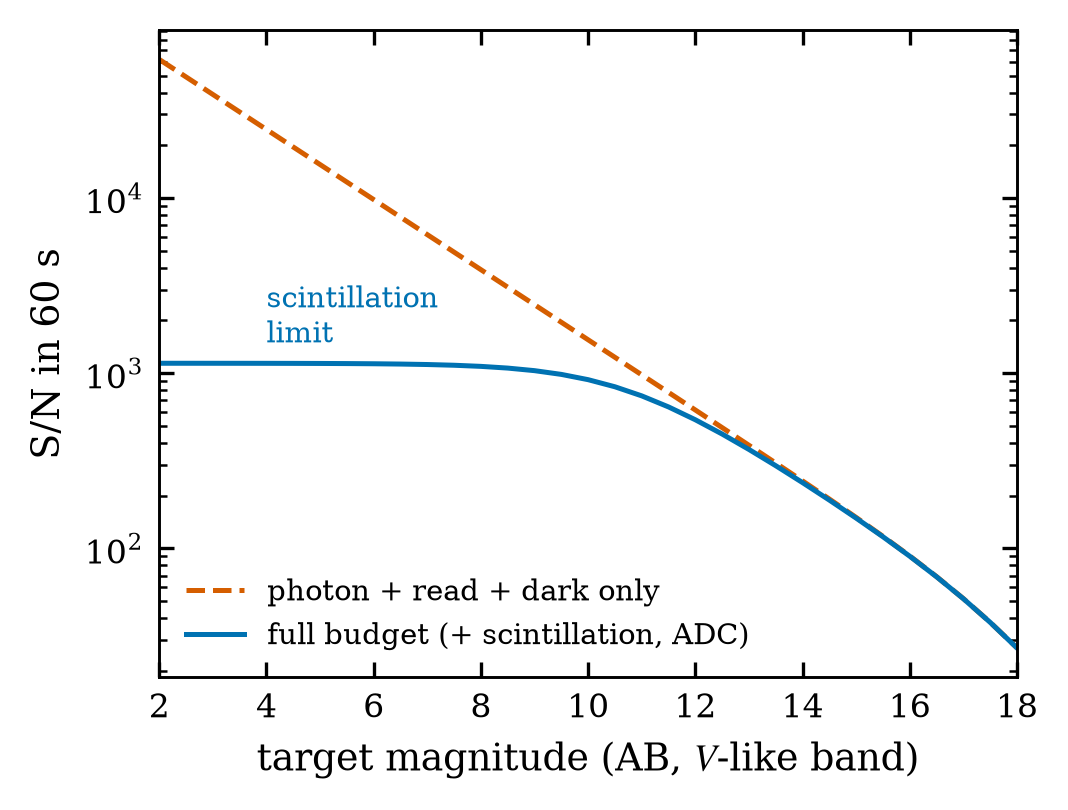
\includegraphics[width=0.62\textwidth]{figures/fig_06_snr_budget.png}
  \caption{Broad-band S/N in \SI{60}{s} for the 358-mm reference
  configuration, computed by the released code. The full budget
  (solid) saturates at the scintillation ceiling
  $\simeq 1.2\times10^{3}$; a Poisson-only model (dashed) overestimates
  bright-star performance by more than an order of magnitude.}
  \label{fig:snrbudget}
\end{figure}

\section{Spectroscopic ETC}
\label{sec:spectroscopy}

Spectroscopy divides the same photons that photometry collects into
hundreds or thousands of wavelength bins, so its S/N per bin is lower by
$\sqrt{N_{\rm bins}}$-like factors and every loss mechanism bites harder.
Two geometries are modelled, and they fail in opposite ways. A
\emph{slit} spectrograph defines its resolution optically and pays for it
at the entrance: slit losses, extraction losses, and --- unless the slit
tracks the parallactic angle --- chromatic losses from atmospheric
dispersion that can silently remove half the blue signal. A
\emph{slitless} grating (the Star Analyser class) pays nothing at an
entrance it does not have, collects every photon of source \emph{and}
sky at every wavelength, and instead surrenders resolution to the
seeing: its resolution element is the star image itself, dispersed. The
engine treats both with the same per-element bookkeeping so that their
trade-off can be compared honestly for the same hardware.

All spectroscopic quantities are per resolution element (``resel''): the
wavelength interval $\Delta\lambda$ the instrument cannot subdivide, one
output row of the ETC. The wavelength grid
is logarithmic at constant $R$ in slit mode, or linear with the resolution
element $\Delta\lambda = \mathcal{D}\,\ell$ in slitless mode
($\mathcal{D}$ = dispersion in \si{\angstrom}/pixel, $\ell$ = LSF FWHM in
pixels). Source and sky rates follow Eq.~(\ref{eq:rate}) restricted to each
element, and the S/N applies Eq.~(\ref{eq:snr}) with
$N_{\rm pix}$ = (dispersion pixels per element) $\times$ (spatial extraction
pixels).

\subsection{Per-element integration: why bin integrals, not samples}
\label{sec:binint}

How the template flux is booked into resolution elements decides whether
line spectroscopy is trustworthy. Sampling the template at the element's
central wavelength and multiplying by $\Delta\lambda$ — the obvious
shortcut — is correct only for spectra smooth on the scale of
$\Delta\lambda$. For a spectral \emph{line} narrower than the element it
is wrong in a way that depends on luck: the line is fully counted if a
sample lands on it and lost if none does, so the \emph{total} detected
line flux changes with the chosen $R$ — unphysical, since dispersing the
same photons more or less finely cannot create or destroy them. The
v10.1 audit measured an $8\times$ spread in the detected counts of a
\SI{2}{\angstrom} emission line between $R = 200$ and $R = 20000$ under
point sampling. Since v10.2 each element's source counts are the exact
\emph{integral} of the calibrated template over the element,
\begin{equation}
  \dot S_i \;=\; \eta\,A \int_{\lambda_i - \Delta\lambda_i/2}
  ^{\lambda_i + \Delta\lambda_i/2}
  \flam^{\rm cal}\, T_\lambda\, Q_\lambda\, O_\lambda\,
  T_{\rm atm}^{\,X}\, \frac{\lambda}{hc}\, d\lambda ,
\end{equation}
evaluated for all elements at once by cumulative trapezoidal integration
on the union of the template grid and the element edges (exact for the
piecewise-linear tabulated inputs, and $O(n)$ — a single pass even at
$R = 10^5$). Total line counts are now invariant under $R$ to better
than 0.2\% (regression-tested), and $\sigma(\mathrm{EW})$
(Sect.~\ref{sec:ew}) inherits that reliability.

\subsection{Slit mode}
\label{sec:slit}

The extracted fraction is the product of two couplings of
Eq.~(\ref{eq:slit}): the slit width across dispersion and the finite
extraction height along it. When the slit is \emph{not} at the parallactic
angle of Eq.~(\ref{eq:parallactic}), the differential refraction
$\Delta R(\lambda)$ of Eq.~(\ref{eq:dr}) decentres the PSF in the slit per
wavelength; \spetc{} applies the worst-case geometry (full offset
perpendicular to the slit), reproducing the classical
\citet{filippenko1982} blue-end losses (Fig.~\ref{fig:dispersion}). A
measured slit-width/resolving-power curve, when supplied, overrides the
nominal $R$.

\subsection{Slitless mode and the Star Analyser}
\label{sec:slitless}

In slitless spectroscopy the resolution element is set by the image quality,
not by a slit: $\ell = \sqrt{(s/p)^2 + \ell_0^2 + \ell_{\rm AD}^2}$ combines
seeing, the intrinsic grating LSF and the atmospheric-dispersion smear
within one element ($s$ = seeing FWHM, $p$ = plate scale, $\ell_0$ =
intrinsic LSF in pixels, $\ell_{\rm AD}$ = dispersion smear in pixels).
The sole extraction aperture is the cross-dispersion height.

\paragraph{The slitless sky is a full-bandpass background.} The decisive
physical difference from a slit is what happens to the \emph{sky}.
Dispersing a spatially \emph{uniform} source leaves the detector
illumination uniform: every wavelength of sky lands on every pixel,
merely shifted, and the shifts of a uniform field are invisible. A
slitless pixel therefore receives the sky integrated over the
\emph{entire} grating bandpass,
\begin{equation}
  \dot B_{\rm pix} \;=\; p^2\, \eta\, A\, \varepsilon_g
  \int_{\lambda_{\rm min}}^{\lambda_{\rm max}}
  \mu_\lambda^{\rm sky}\, T_\lambda\, Q_\lambda\, O_\lambda\,
  \frac{\lambda}{hc}\, d\lambda ,
  \label{eq:slitless-sky}
\end{equation}
with $\mu_\lambda^{\rm sky}$ the sky spectral surface brightness per
arcsec$^2$, $p^2$ the pixel solid angle and $\varepsilon_g$ the grating
efficiency; the sky per element is $\dot B_{\rm pix}$ times the
extraction pixels. This is the classical reason objective-grating spectra
are sky-limited. Booking only one element's $\Delta\lambda$ of sky per
pixel — as a slit would allow — underestimates the background by the
ratio (bandpass width)/(element width), about two orders of magnitude for
a Star Analyser covering \SI{3300}{\angstrom} with \SI{28}{\angstrom}
elements; the v10.1 audit measured a $118\times$ deficit, corrected in
v10.2 and regression-tested. Practical consequence: slitless S/N under a
bright sky is far worse than a slit ETC intuition suggests, and the
mode's advantage survives only for short exposures on brighter targets —
which is precisely how Star Analysers are productively used.

For a transmission grating in the converging beam --- the Star Analyser
100/200 geometry --- the first-order deviation is
$x \simeq L\,m\,n\,\lambda$, so the dispersion at the detector is
\begin{equation}
  \mathcal{D} \;=\; \frac{10^{4}\, p_{\mu m}}{L_{\rm mm}\; n_{\rm mm}\; m}
  \quad [\si{\angstrom}/\text{pixel}],
  \label{eq:sa}
\end{equation}
with $n$ the groove density (100 or 200 mm$^{-1}$), $L$ the
grating-to-sensor distance and $m=1$. An SA100 at $L=\SI{42}{mm}$ on
\SI{4.63}{\micro\metre} pixels gives $\mathcal{D} = 11.0$
\si{\angstrom}/pixel, matching its published calibration; an SA200 at the
same distance gives half that. An optional scalar first-order grating
efficiency multiplies source and sky alike. Under $2.5''$ seeing the
effective resolving power is $R \simeq 100$--200
(Fig.~\ref{fig:sa100}), which is why the mode remains flagged
\emph{experimental} until validated against a calibrated instrument.

\begin{figure}
  \centering
  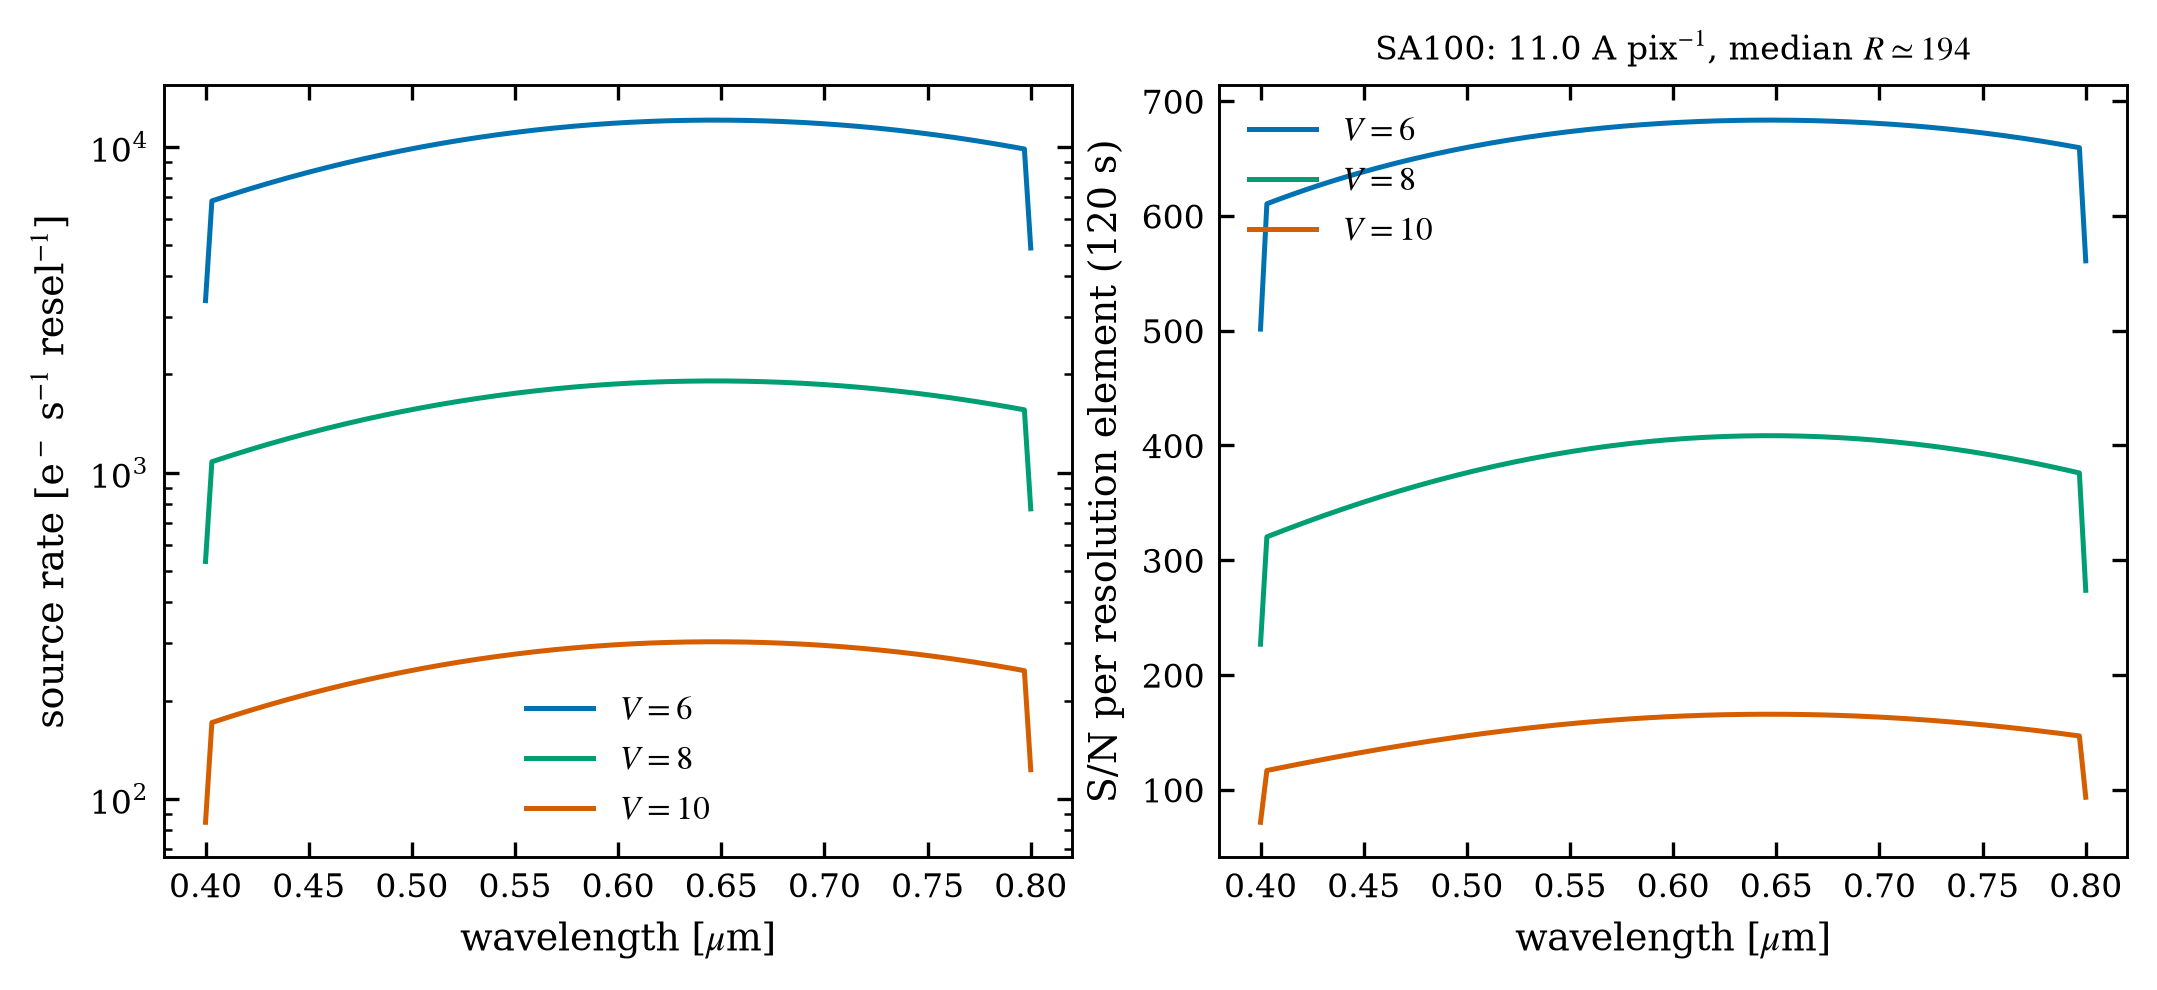
\includegraphics[width=\textwidth]{figures/fig_07_sa100.png}
  \caption{Star Analyser 100 predictions from the released code for a
  200-mm f/5 telescope with a typical CMOS camera: detected source rate
  (left) and S/N per resolution element in \SI{120}{s} (right) for
  $V = 6, 8, 10$ flat-spectrum targets.}
  \label{fig:sa100}
\end{figure}

\subsection{Slit-spectrograph geometry}
\label{sec:geometry}

Amateurs know their spectrograph by its hardware — groove density $n$,
collimator and camera focal lengths $f_{\rm coll}, f_{\rm cam}$, slit
width — not by $R$. In the Littrow approximation the grating equation
gives $\sin\beta = m n \lambda/2$ and a reciprocal linear dispersion
$d\lambda/dx = \cos\beta \cdot 10^{7}/(m\,n\,f_{\rm cam})$
[\si{\angstrom}/mm]. The resolution element on the detector is the
narrower of the geometric slit image and the seeing image, both reimaged
by $f_{\rm cam}/f_{\rm coll}$ (anamorphism 1 in Littrow):
\begin{equation}
  \Delta\lambda = \min(w_{\rm slit}, w_{\rm seeing})\,
  \frac{f_{\rm cam}}{f_{\rm coll}}\,\frac{d\lambda}{dx},
  \qquad R = \frac{\lambda}{\Delta\lambda},
\end{equation}
with the widths converted from arcsec at the telescope focal plane. The
calculator reports whether the configuration is slit- or seeing-limited
and feeds the ETC's resolving-power field, which remains editable; an
LHIRES III-like configuration (2400 lines/mm, $f=200$~mm Littrow, 25-\si{\micro\metre}
slit) returns $R \simeq 2\times10^4$ at H$\alpha$, in line with the
instrument's specification.

Two guards keep the entered $R$ honest (v10.2). With the geometry
supplied and the clamp option enabled, the engine itself limits the
entered $R$ to the geometry's value at the band centre — a physically
impossible $R$ can then no longer silently inflate every per-element
prediction. Conversely, when the seeing disc is much \emph{narrower}
than the slit the delivered resolution is set by the star image, i.e.\
finer than the slit-limited $R$; the engine flags this case so the user
knows the reported $R$ is conservative.

\subsection{Equivalent-width detectability}
\label{sec:ew}

The spectroscopic S/N is turned into a science answer through the
\citet{cayrel1988} relation for the equivalent-width uncertainty of a line
of FWHM $W$ sampled with pixels of width $\delta x$:
\begin{equation}
  \sigma(\mathrm{EW}) \;\simeq\; \frac{1.5\,\sqrt{W\,\delta x}}
  {(\mathrm{S/N})_{\rm pixel}},
  \label{eq:cayrel}
\end{equation}
evaluated per wavelength with the resolution element as $W$ and reported
in m\AA{} in every result table. The practical criterion: a line is
securely measurable when its expected equivalent width exceeds
$\simeq 3\,\sigma(\mathrm{EW})$ — e.g.\ $\sigma(\mathrm{EW}) = 15$~m\AA{}
means H$\alpha$ variations of a Be star at the 50~m\AA{} level are
detectable, while 20~m\AA{} photospheric lines are marginal.

\subsection{Time series and reverse solving}

Planning series evaluate the S/N reference wavelength bin at every time
sample of the visibility window (full spectra only at the selected time and
the plot-slider samples), with the sky model, airmass, refraction and
parallactic angle recomputed per sample. Target-S/N requests use the
closed-form solver of Sect.~\ref{sec:noise} per element and are checked
against the saturation limit rather than being silently declared feasible.

\section{Filter profiles and synthetic calibration}
\label{sec:filters}

Professional passbands (Johnson--Cousins, Sloan, 2MASS, \dots) ship as SVO
Filter Profile Service VOTables \citep{rodrigo2020}. Amateur filters
(Astrodon, Astronomik, Baader, Optolong, Chroma RGB and narrowband sets)
are absent from SVO, but a measured or digitized transmission curve is all
that is required: the zero points are \emph{computed}, not measured. The
bundled \code{make\_filter\_profile.py} applies the same synthetic
convention SVO itself uses:
\begin{itemize}
\item \textbf{AB}: $Z_\nu = \SI{3631}{Jy}$ at every wavelength by
  definition \citep{oke1983};
\item \textbf{Vega}: the photon-weighted mean flux density of the CALSPEC
  Vega spectrum \citep{bohlin2014} through the filter,
  \begin{equation}
    Z_\nu \;=\; \frac{\displaystyle\int F_\lambda^{\rm Vega}\,
    T_\lambda\,\lambda\,d\lambda}
    {\displaystyle\int \frac{c}{\lambda^2}\,T_\lambda\,\lambda\,d\lambda},
  \end{equation}
  i.e.\ the flux a magnitude-zero star delivers in this band.
\end{itemize}
The tool writes full SVO-format VOTables with the complete photdm
annotation and every characterising quantity measured from the curve by
the SVO definitions (mean, pivot, effective and photon-weighted
wavelengths, 1\%-of-peak limits, effective width, FWHM, and the mean solar
flux \code{Fsun} from the CALSPEC solar spectrum), so the produced files
are drop-in interchangeable with SVO downloads and land on exactly the
same photometric scale as the shipped professional profiles.

\begin{table}
\centering
\caption{Validation of the synthetic calibration against the shipped SVO
2MASS.H profile (whose declared values are independent of this code).}
\label{tab:filtercal}
\begin{tabular}{lccc}
\toprule
Quantity & SVO declared & Computed here & Difference \\
\midrule
Pivot wavelength [\si{\angstrom}] & 16494.9 & 16494.7 & $-0.00\%$ \\
Photon-weighted wavelength [\si{\angstrom}] & 16460.6 & 16423.8 & $-0.2\%$ \\
Central wavelength [\si{\angstrom}] & 16506.1 & 16487.3 & $-0.1\%$ \\
$F_\odot$ [\si{erg.cm^{-2}.s^{-1}.\angstrom^{-1}}] & 22.44 & 22.33 & $-0.5\%$ \\
Vega zero point [Jy] & 1024.0 & 1030.4 & $+0.6\%$ \\
\bottomrule
\end{tabular}
\end{table}

Table~\ref{tab:filtercal} validates the pipeline end-to-end on 2MASS.H:
the sub-percent agreement (the residuals reflect SVO's slightly different
Vega SED normalization) means a profile built from a digitized Astrodon or
Astronomik curve is calibrated to the same standard as a professional
filter — no laboratory measurement beyond the transmission curve itself is
needed.

\section{Expected performance and limits of validity}
\label{sec:expectations}

\subsection{What to expect}

\begin{itemize}
\item \textbf{Bright stars are scintillation-limited.} For the 358-mm
  reference telescope, a $V\simeq5$ star in \SI{60}{s} reaches
  $\mathrm{S/N}\simeq1.3\times10^{3}$, not the $\sim2\times10^{4}$ a
  photon-only budget would claim (Fig.~\ref{fig:snrbudget}); the ceiling
  scales as $d^{2/3} X^{-1.75} \sqrt{t}$.
\item \textbf{Faint limits are sky-limited.} Beyond
  $m \gtrsim \mu_{\rm sky} - 2.5\log_{10}(\pi r^2)$ the S/N falls as
  $10^{-0.4m}$ and doubling the exposure gains only $\sqrt{2}$.
\item \textbf{Moonlight matters within $\sim90^\circ$.} Full Moon at
  $30^\circ$ separation brightens the $V$ sky by $\simeq4$--5 mag
  (Sect.~\ref{sec:sky}), turning background-limited exposures from minutes
  into hours.
\item \textbf{Slit spectroscopy away from the parallactic angle} loses tens
  of per cent at the blue end already at $X = 1.5$--2
  (Fig.~\ref{fig:dispersion}); the Results window reports $q$ at every
  sample so the slit can be set correctly.
\item \textbf{Star Analyser work} is photometrically generous (no slit
  losses) but limited to $R\sim100$--200 by seeing; S/N per element of
  several hundred in minutes is realistic for $V \lesssim 8$
  (Fig.~\ref{fig:sa100}).
\end{itemize}

\subsection{Known approximations}

The model is explicit about its accuracy floor: the $U$--$K$ sky table and
its colour interpolation are broad-band, and the twilight/daylight bridge is
approximate; the extinction fallback table is a smooth broad-band baseline
until a site-specific curve is loaded; scintillation uses the classical
Young coefficient (site-specific coefficients from \citealt{osborn2015} can
be substituted); atmospheric dispersion in slit mode assumes the worst-case
orientation; extended sources are uniform discs; and slitless mode awaits
validation against a calibrated instrument. Flat-field and fringing
residuals, cosmic rays and sky-subtraction penalties are not modelled.

\subsection{Numerical verification}

Two test programs ship with the code: a synthetic smoke test that pins the
scintillation-limited photometric S/N and the per-element spectroscopic S/N
of the reference configuration, and a regression suite that verifies, among
others, Eq.~(\ref{eq:ks}) against the published scattering function, the
ecliptic symmetry of the zodiacal term, Eq.~(\ref{eq:pickering}) against
$\sec z$, the Student-$t$ Moffat coupling, the Filippenko dispersion scale,
Eq.~(\ref{eq:sa}) for the SA100/SA200, and the extended-source area
fractions.

\section{A worked example, by hand}
\label{sec:example}

To connect the formulae to the numbers the program prints, this section
computes one photometric case almost entirely by hand: a $V = 12.0$
(Vega) solar-type star, observed in $V$ through a 200-mm f/5 Newtonian
(secondary obstruction 70\,mm, optics efficiency 0.85) with a typical
CMOS camera (QE $\simeq 0.8$ at 5500\,\AA{}, gain setting giving
1.0\,e$^-$/ADU, read noise 1.5\,e$^-$, pixel 3.76\,\si{\micro\metre}),
under $2.5''$ seeing at airmass 1.2 from a suburban site
(SQM = 20.0, elevation 300\,m), for 60\,s in a $5''$-radius aperture.

\paragraph{1. Photon budget of the source.} A $V=0$ star delivers about
$1.0\times10^{4}$ photons\,s$^{-1}$\,cm$^{-2}$\,\AA$^{-1}$... more
precisely, Eq.~(\ref{eq:flam}) with $Z_\nu = 3640$\,Jy at 5500\,\AA{}
gives $F_\lambda = 3.63\times10^{-9}$\,erg\,s$^{-1}$cm$^{-2}$\AA$^{-1}$,
i.e.\ $F_\lambda/(hc/\lambda) \simeq 1005$
photons\,s$^{-1}$cm$^{-2}$\AA$^{-1}$. At $V=12$: $\times10^{-0.4\cdot12}
= 1.58\times10^{-5}$, so $1.59\times10^{-2}$
photons\,s$^{-1}$cm$^{-2}$\AA$^{-1}$.

\paragraph{2. Collecting area and effective bandwidth.} $A = \pi(20.0^2 -
7.0^2)/4 = 275.7$\,cm$^2$. The Bessell $V$ band has an effective width
of $\simeq 870$\,\AA{}. Through atmosphere ($T^X \simeq 0.87^{1.2}
\simeq 0.85$ at $V$), optics (0.85) and QE (0.80):
\[
\dot S_{\rm tot} \simeq 1.59\times10^{-2} \times 275.7 \times 870
\times 0.85 \times 0.85 \times 0.80 \;\simeq\; 2.2\times10^{3}\;
\mathrm{e^-\,s^{-1}} .
\]
The program, integrating the real solar-type spectrum against the real
$V$ curve, reports $\simeq 2.1\times10^{3}$\,e$^-$/s --- the hand
estimate is good to ten percent, which is the accuracy of using an
effective width.

\paragraph{3. Aperture and sky.} A $5''$ radius is $2\times$ the seeing
FWHM: a Moffat ($\beta=2.5$) profile puts 89\% of the light inside
(Sect.~\ref{sec:psf}), so $\dot S = 0.89 \times 2100 \simeq 1.9\times10^{3}$
e$^-$/s, and $S = 1.1\times10^{5}$\,e$^-$ in 60\,s. The aperture covers
$\pi\,25 = 78.5$\,arcsec$^2$. SQM 20.0 means the sky is
$m_{\rm sky} = 20.0$ mag/arcsec$^2$ in $V$, i.e.\ per arcsec$^2$ the sky
is a $20.0$-mag source: $\dot B = 2100 \times 10^{-0.4(20.0-12.0)}
\times 78.5 \simeq 2.6\times10^{2}$\,e$^-$/s, $B = 1.6\times10^{4}$
e$^-$ in 60\,s. With a plate scale of $0.776''$/pixel the aperture
holds $N_{\rm pix} \simeq 130$ pixels.

\paragraph{4. Noise budget.} Shot noise: $\sqrt{S + B} =
\sqrt{1.1\times10^5 + 1.6\times10^4} = 355$\,e$^-$. Read:
$\sqrt{130}\times1.5 = 17$\,e$^-$. Quantization:
$\sqrt{130}\times 1.0/\sqrt{12} = 3$\,e$^-$. Scintillation,
Eq.~(\ref{eq:scint}): $\sigma/I = 0.09\times20^{-2/3}\times1.2^{1.75}
\times e^{-300/8000}/\sqrt{120} = 1.5\times10^{-3}$, so
$\sigma_{\rm scint} = 1.5\times10^{-3}\times1.1\times10^{5} =
165$\,e$^-$. Total: $\sqrt{355^2 + 165^2 + 17^2 + 3^2} = 392$\,e$^-$.

\paragraph{5. Result.} $\mathrm{S/N} = 1.1\times10^{5}/392 \simeq 280$
--- a differential precision of $1086/280 \simeq 3.9$\,mmag per frame
against an equal comparison star ($\times\sqrt2$: 5.5\,mmag), fine for
a 25-mmag exoplanet transit at two-minute cadence. Note where the noise
lives: shot noise dominates, but scintillation is already 42\% of it at
$V=12$ on a 20-cm aperture --- brighten the star by three magnitudes
and scintillation rules alone, which is why the S/N curve of
Fig.~\ref{fig:snrbudget} flattens. The peak pixel holds
$\simeq 2100\times0.07\times60 \simeq 9\times10^{3}$\,e$^-$
(central-pixel fraction 0.07 for this sampling) plus sky and dark ---
far from a CMOS full well at low gain, so the 60-s frame is safe, as the
program's saturation columns confirm.

Every number above is printed by one run of the program; the exercise
shows there is no magic between the inputs and the outputs --- only the
chain of Sect.~\ref{sec:chain}, executed carefully.


\bibliography{references}

\end{document}
